\documentclass[conference]{IEEEtran}
\usepackage{graphicx}
\usepackage{amsmath,amssymb}
\usepackage{booktabs}
\usepackage{cite}
\usepackage{url}
\usepackage{placeins}
\usepackage{tikz}
\usetikzlibrary{arrows.meta,positioning}
\begin{document}
\title{Vision-Based Object Discovery in ROS 2--Gazebo: A 51-Trial Evaluation of Assisted DDQN and PPO Versus Random Exploration}
\author{\IEEEauthorblockN{THATIPAMULA GRANTHIK RANADHEER}
\IEEEauthorblockA{Department of Computer Science and Engineering (CSE)\\
Indian Institute of Information Technology, Sri City\\
Andhra Pradesh, India\\
granthikranadheer.t24@iiits.in}}
\maketitle
\begin{abstract}
Autonomous object discovery couples navigation with imperfect perception: a mobile robot must acquire views of distinct targets while avoiding repeated coverage and obstacles. This paper evaluates a ROS 2 Humble and Gazebo 11 system with a simulated TurtleBot3 Burger, 360-beam LiDAR, RGB--depth sensing, a fine-tuned YOLO11n detector, and world-frame instance matching. The final world contains 26 target instances in an 18\,m by 18\,m bounded region. We analyze original records from 17 trials each for deterministic Double Deep Q-Network (DDQN) and Proximal Policy Optimization (PPO) policies supplemented by map-based coverage, inspection, and safety routines, and for unassisted uniform-random exploration. Each trial used one of the same 17 seeds and ended at 26 matches or 12 minutes. Mean counts were 25.41, 25.24, and 19.35 for DDQN, PPO, and Random; full-discovery counts were 11/17, 9/17, and 1/17. Among successful trials, mean completion times were 3.02, 3.05, and 6.94 minutes. Only 3.4\% and 3.3\% of DDQN and PPO logged actions, respectively, were applied directly from their policies; other actions came from assistance. Thus, the results compare complete evaluated control configurations in one simulated world, rather than establish intrinsic superiority of a learning algorithm. We quantify variability and right-censored completion and discuss limitations of matching detections to the 26 target instances.
\end{abstract}
\begin{IEEEkeywords}
robotic exploration, object discovery, ROS 2, Gazebo, YOLO, Double DQN, PPO, mobile robots
\end{IEEEkeywords}

\section{Introduction}
A mobile robot searching for objects must move through a partially observed environment, acquire useful camera views, and distinguish new instances from repeated detections. Frontier exploration drives a robot toward boundaries of mapped and unmapped space~\cite{yamauchi1997}; learned exploration and semantic vision offer alternative ways to select informative actions~\cite{chaplot2020}. Object discovery is stricter than geometric coverage: traversing a location does not guarantee recognition of a small, occluded, or misclassified object.

Our question is: \emph{How do the final evaluated DDQN-based, PPO-based, and random exploration configurations compare in matched-object coverage and completion time in a controlled ROS 2--Gazebo world?} The term \emph{configuration} matters. Both learned policies were embedded in map-based coverage and inspection controllers, while Random used sampled actions alone. The study therefore measures delivered systems, not a controlled policy-only contrast.

The contributions are: (i) an auditable ROS 2 perception--control--evaluation pipeline combining RGB--depth detections with robotic exploration; (ii) a final 26-instance world and 51 recorded, seed-aligned, time-limited trials; and (iii) an analysis of coverage, completion, time, object-level misses, and the source of applied actions. We do not propose a new reinforcement-learning algorithm or claim physical-robot testing.

\section{Related Work}
Frontier-based exploration selects reachable boundaries of an occupancy map~\cite{yamauchi1997}. Learned exploration systems can combine mapping and policy modules, as in Active Neural SLAM~\cite{chaplot2020}. These works motivate considering map-derived action selection when interpreting a learned controller.

Deep Q-learning introduced neural action-value approximation and replay~\cite{mnih2015}. Double DQN separates online action selection from target-network evaluation to reduce Q-value overestimation~\cite{vanhasselt2016}. PPO instead improves an actor--critic policy using a clipped probability-ratio objective~\cite{schulman2017}. Stable-Baselines3 provides the base implementations used here~\cite{raffin2021}. Neither algorithm specifies the perception, safety, or coverage controller around it.

YOLO predicts classes and boxes from an image~\cite{redmon2016}; the deployed principal model is an Ultralytics YOLO11n variant~\cite{ultralyticsmodels}. ROS 2 provides message passing~\cite{macenski2022}; Gazebo simulates sensing and dynamics~\cite{koenig2004}; and SLAM Toolbox supplies the occupancy map used by assisted configurations~\cite{macenski2021slam}. This paper examines the joint behavior of those components and audits the effective control mix.

\section{System Architecture}
\subsection{Simulation and Robot}
The final experiment uses Gazebo Classic 11.10.2, an SDF 1.6 world, and ROS 2 Humble. The simulated TurtleBot3 Burger has differential drive, odometry, a 360-sample planar LiDAR (0.12--3.5\,m), and a depth camera (about 60-degree horizontal field of view, 0.10--10\,m depth limits). The model publishes \texttt{/scan}, \texttt{/odom}, \texttt{/camera/rgb/image\_raw}, and \texttt{/camera/depth/points}; motion arrives on \texttt{/cmd\_vel}. No physical sensors were tested.

Four walls bound the world at $x=\pm9$\,m and $y=-11,7$\,m. The robot starts at $(0,-2)$\,m. The 26 scored SDF includes comprise two person instances, point-cloud-derived bottle and doll models, a cabinet, and other everyday or industrial objects. Their model origins span $x=-7$ to $7$\,m and $y=-9$ to $4.6$\,m; ten have origin height above 0.10\,m. The cabinet is a physical obstacle and a scored target because it is an included model. Figure~\ref{fig:gazebo26} shows a new Gazebo capture of the final world used in all 51 trials, obtained outside the timed trials. The Hokuyo laser-ray \emph{visualization} was disabled only for this capture to remove blue ray fans; the target layout and model geometry were unchanged. Figure~\ref{fig:layout} is a coordinate-derived schematic of that world. Neither illustration is a trial outcome. The display stands and boundary walls are environment structures, not scored targets. Table~\ref{tab:inventory} lists every scored instance, its SDF pose, its scored class, and the frequency of a match in each 17-trial series.

\paragraph{Model provenance.} The 24 non-PCD target models were taken from the Open Robotics (OSRF) Gazebo model database at \url{https://github.com/osrf/gazebo_models}, local checkout \texttt{8163eb4b5e7e21985c6591d1c0bfb56468c0093f}~\cite{osrfmodels}. Their individual \texttt{model.config} files retain model-author metadata. The remaining two target models, \texttt{pcd\_bottle} and \texttt{pcd\_doll}, were generated locally by \texttt{create\_pcd\_gazebo\_models.py} from \texttt{bottle.pcd} and \texttt{doll.pcd} already present in the project workspace; an external source URL for those original point clouds was not recorded. The assembled world is \texttt{src/robot\_tasks/worlds/spaced\_objects\_reliable\_26\_v4.world}; it and the conversion code are in the project repository~\cite{projectrepo}. These are 26 scored \emph{instances}, not necessarily 26 distinct detector classes.

\begin{table*}[t]
\caption{The 26 scored object instances in the final SDF world. Positions are SDF model origins in metres, rounded to two decimals. DDQN (D), PPO (P), and Random (R) give the number of trials (out of 17) that matched each instance. IDs correspond to Figs.~\ref{fig:layout} and \ref{fig:objectfreq}.}
\label{tab:inventory}
\centering\scriptsize
\setlength{\tabcolsep}{3pt}
\begin{tabular}{@{}rllrrrrrr@{}}
\toprule
ID & SDF instance & Scored class & $x$ & $y$ & $z$ & D & P & R \\ \midrule
1 & \texttt{table\_main} & \texttt{table} & -2.50 & -5.60 & 0.00 & 16 & 17 & 12 \\
2 & \texttt{person\_standing\_main} & \texttt{person} & 4.20 & -9.00 & 0.00 & 17 & 17 & 14 \\
3 & \texttt{person\_walking\_main} & \texttt{person} & 1.80 & -6.80 & 0.00 & 17 & 17 & 15 \\
4 & \texttt{construction\_barrel\_object} & \texttt{construction\_barrel} & -7.00 & -6.20 & 0.00 & 17 & 17 & 12 \\
5 & \texttt{mailbox\_object} & \texttt{mailbox} & 7.00 & -6.20 & 0.00 & 16 & 16 & 13 \\
6 & \texttt{postbox\_object} & \texttt{postbox} & -7.00 & -3.40 & 0.00 & 17 & 17 & 14 \\
7 & \texttt{stop\_sign\_object} & \texttt{stop\_sign} & -3.20 & 1.10 & 0.00 & 17 & 17 & 14 \\
8 & \texttt{lamp\_post\_object} & \texttt{lamp\_post} & -7.00 & -0.60 & 0.00 & 17 & 14 & 13 \\
9 & \texttt{grey\_tote\_object} & \texttt{grey\_tote} & 3.50 & 4.60 & 0.03 & 15 & 14 & 8 \\
10 & \texttt{bowl\_object} & \texttt{bowl} & 0.00 & -4.00 & 0.36 & 17 & 17 & 13 \\
11 & \texttt{drill\_object} & \texttt{cordless\_drill} & 4.20 & -6.20 & 0.36 & 16 & 16 & 15 \\
12 & \texttt{hammer\_object} & \texttt{hammer} & -0.60 & -1.00 & 0.36 & 17 & 17 & 10 \\
13 & \texttt{beer\_object} & \texttt{beer} & -1.40 & -3.40 & 0.24 & 17 & 17 & 14 \\
14 & \texttt{fire\_hydrant\_object} & \texttt{fire\_hydrant} & 1.40 & -3.40 & 0.00 & 17 & 17 & 15 \\
15 & \texttt{construction\_cone\_object} & \texttt{construction\_cone} & 4.20 & -3.40 & 0.00 & 17 & 17 & 14 \\
16 & \texttt{cardboard\_box\_object} & \texttt{cardboard\_box} & -4.20 & -0.60 & 0.15 & 17 & 17 & 14 \\
17 & \texttt{cricket\_ball\_object} & \texttt{cricket\_ball} & 0.50 & 0.50 & 0.40 & 16 & 16 & 9 \\
18 & \texttt{monkey\_wrench\_object} & \texttt{monkey\_wrench} & 1.40 & -0.60 & 0.36 & 15 & 14 & 11 \\
19 & \texttt{car\_wheel\_object} & \texttt{car\_wheel} & 4.20 & -0.60 & 0.08 & 17 & 17 & 15 \\
20 & \texttt{hokuyo\_object} & \texttt{hokuyo} & -1.25 & -2.42 & 0.40 & 17 & 17 & 9 \\
21 & \texttt{wooden\_case\_object} & \texttt{wooden\_case} & -1.40 & 2.20 & 0.02 & 17 & 17 & 13 \\
22 & \texttt{saucepan\_object} & \texttt{saucepan} & 1.40 & 2.20 & 0.39 & 16 & 17 & 10 \\
23 & \texttt{gear\_part\_object} & \texttt{gear\_part} & 0.20 & -1.20 & 0.36 & 16 & 16 & 10 \\
24 & \texttt{bottle\_pcd\_object} & \texttt{bottle} & -0.56 & -3.35 & 0.00 & 17 & 17 & 13 \\
25 & \texttt{doll\_pcd\_object} & \texttt{doll} & 1.68 & -2.34 & 0.00 & 17 & 17 & 14 \\
26 & \texttt{cabinet\_main} & \texttt{cabinet} & 4.00 & -2.00 & 0.00 & 17 & 17 & 15 \\
\bottomrule
\end{tabular}
\end{table*}

\begin{figure*}[t]
\centering
\resizebox{0.96\textwidth}{!}{%
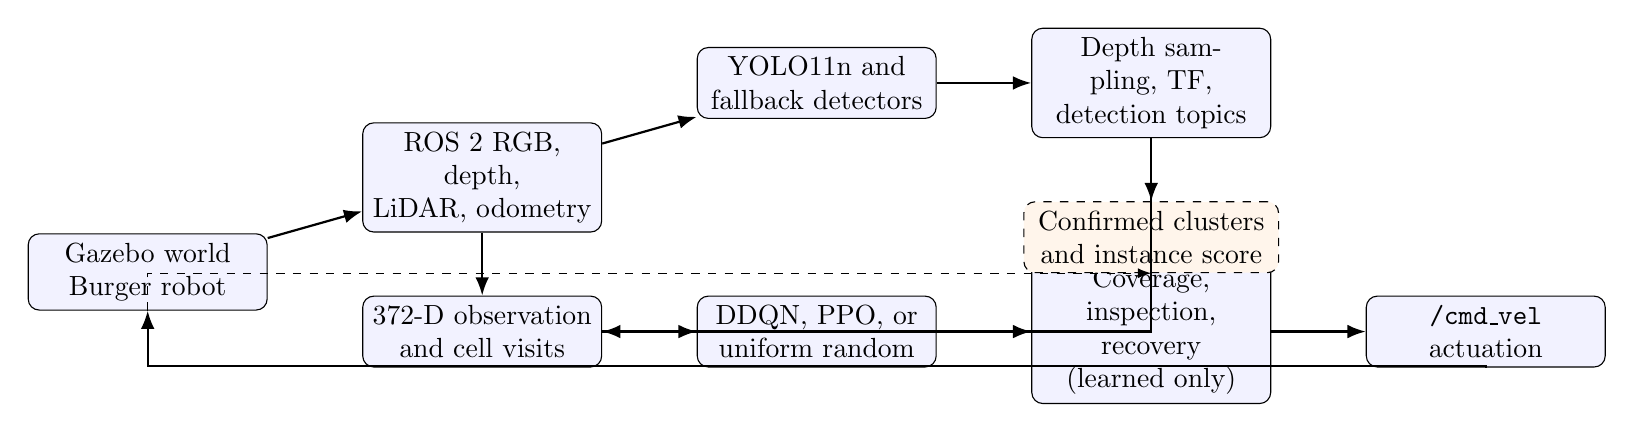
\begin{tikzpicture}[>=Latex,node distance=8mm and 12mm,
box/.style={draw,rounded corners,fill=blue!5,align=center,minimum height=9mm,text width=28mm},
score/.style={draw,dashed,rounded corners,fill=orange!8,align=center,minimum height=9mm,text width=30mm}]
\node[box] (gaz) {Gazebo world\\Burger robot};
\node[box,right=of gaz,yshift=12mm] (sensor) {ROS 2 RGB, depth,\\LiDAR, odometry};
\node[box,right=of sensor,yshift=12mm] (yolo) {YOLO11n and\\fallback detectors};
\node[box,right=of yolo] (xyz) {Depth sampling, TF,\\detection topics};
\node[box,below=of sensor] (obs) {372-D observation\\and cell visits};
\node[box,right=of obs] (pol) {DDQN, PPO, or\\uniform random};
\node[box,right=of pol] (assist) {Coverage, inspection,\\recovery (learned only)};
\node[box,right=of assist] (cmd) {\texttt{/cmd\_vel}\\actuation};
\node[score,below=of xyz] (eval) {Confirmed clusters\\and instance score};
\draw[->,thick] (gaz)--(sensor);
\draw[->,thick] (sensor)--(yolo);
\draw[->,thick] (yolo)--(xyz);
\draw[->,thick] (sensor)--(obs);
\draw[->,thick] (xyz)|-(obs);
\draw[->,thick] (obs)--(pol);
\draw[->,thick] (pol)--(assist);
\draw[->,thick] (assist)--(cmd);
\draw[->,thick] (cmd.south)|-([yshift=-7mm]gaz.south)--(gaz.south);
\draw[->,thick] (xyz)--(eval);
\draw[->,dashed] (gaz.south)|-(eval.south);
\end{tikzpicture}}
\caption{Implemented data flow. The dashed world-pose path is restricted to scoring; the coverage planner uses SLAM map and visit history, not target poses. Assistance is disabled for Random.}
\label{fig:architecture}
\end{figure*}

\begin{figure*}[t]
\centering
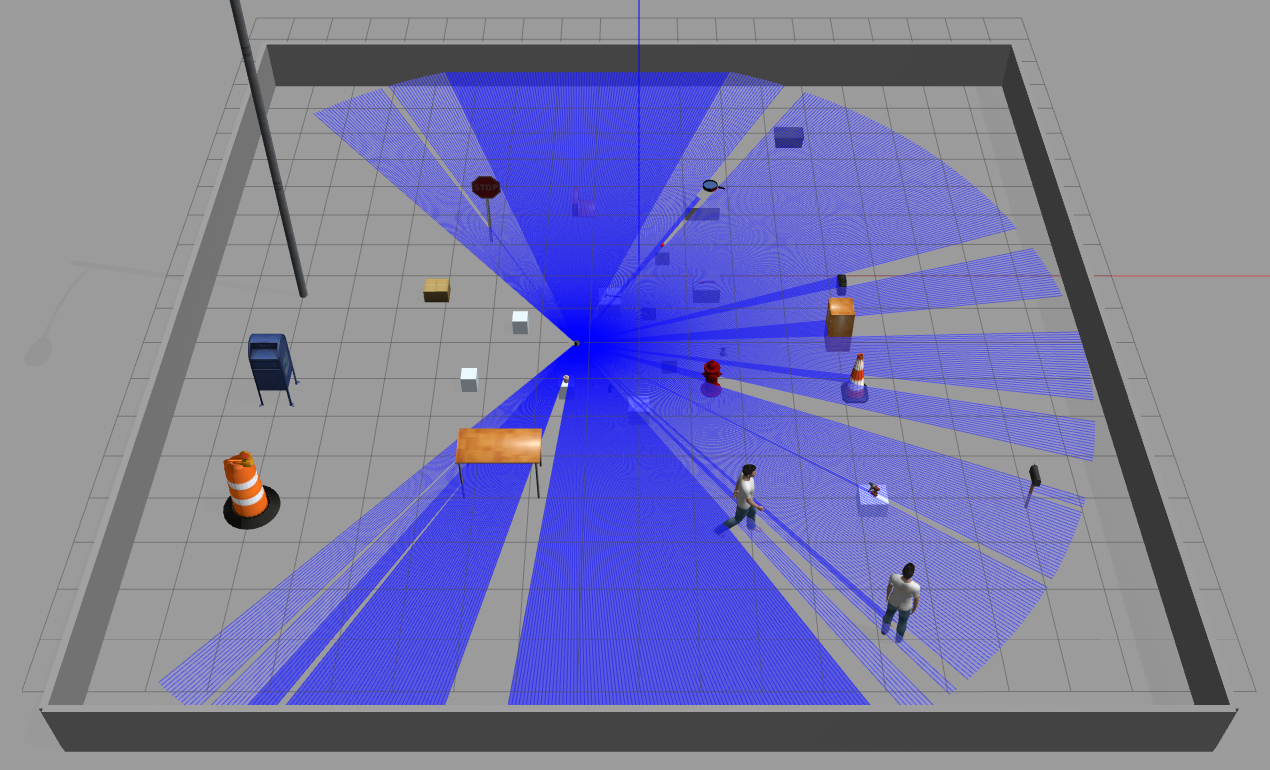
\includegraphics[width=0.82\textwidth]{figures/gazebo_26_object_world.png}
\caption{Gazebo Classic view of the final 26-target SDF world, captured separately from the 51 timed trials. Hokuyo laser-ray visualization was switched off for this image only; object geometry and placement were unchanged. Target positions are listed in Table~\ref{tab:inventory}.}
\label{fig:gazebo26}
\end{figure*}

\begin{figure*}[t]
\centering
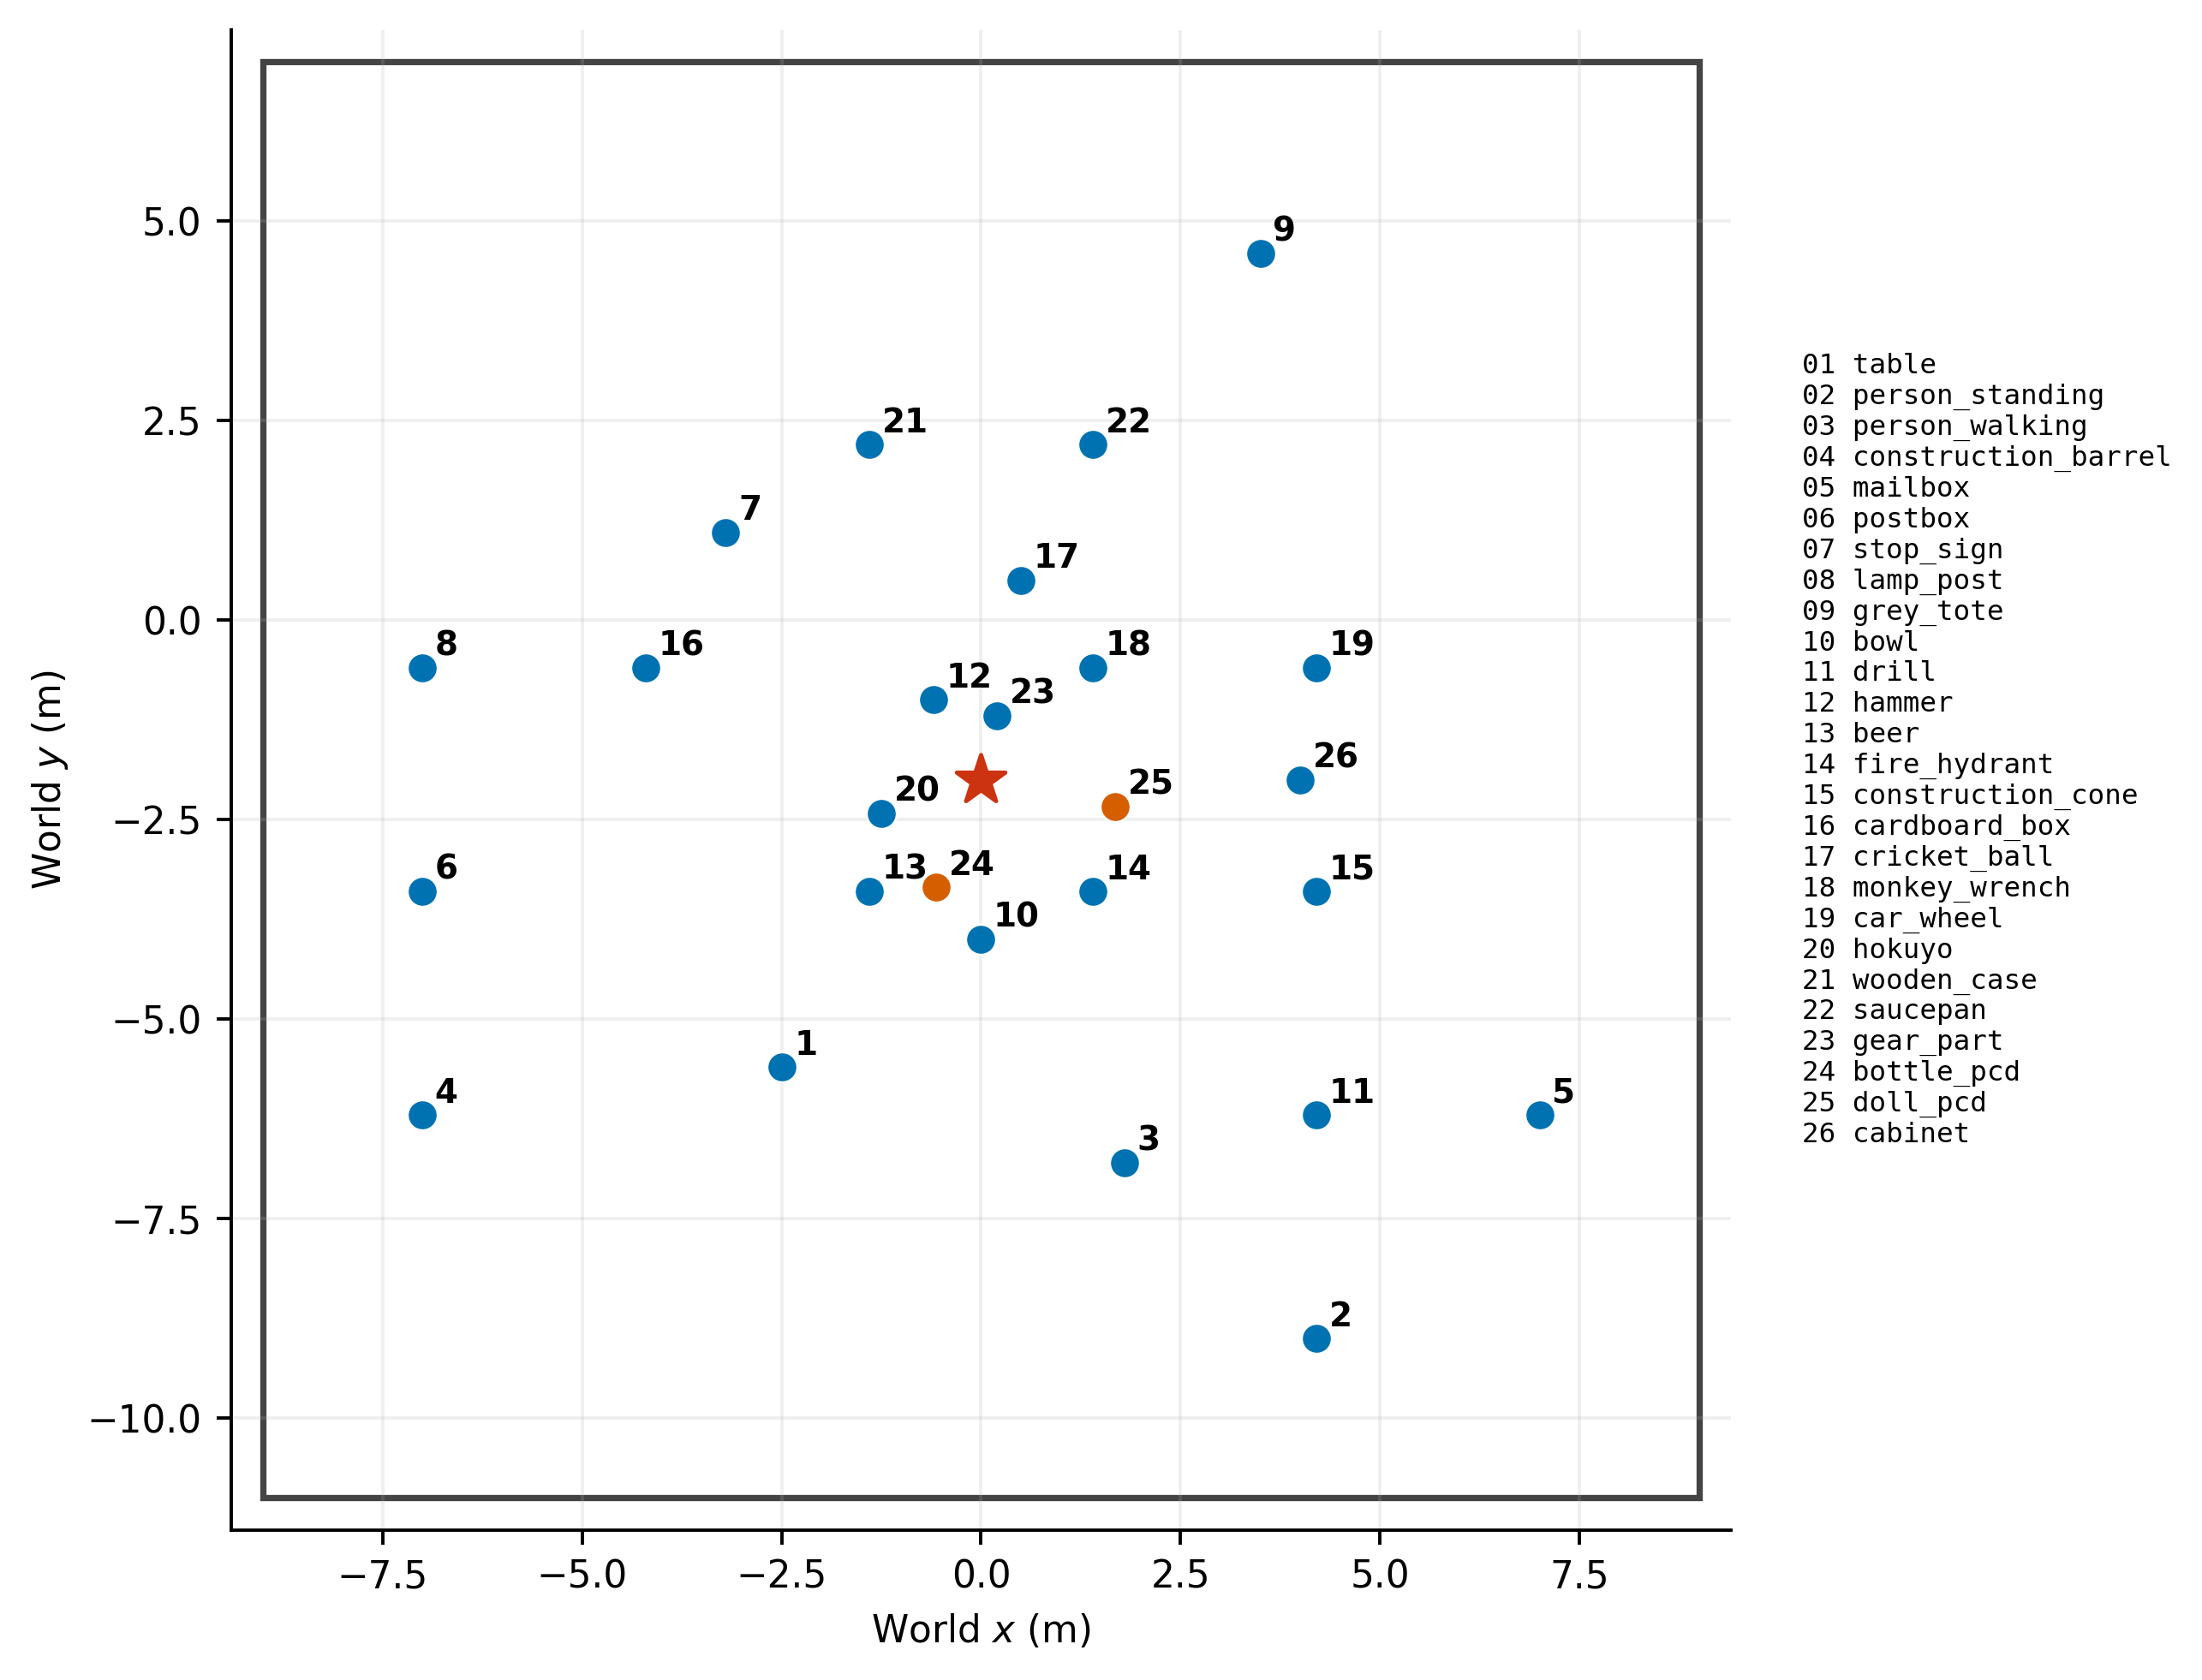
\includegraphics[width=0.94\textwidth]{figures/environment_layout.png}
\caption{Schematic from the final SDF world. Numbers correspond to the 26 scored instances in Table~\ref{tab:inventory}; the star marks robot start, and orange points mark the bottle and doll point-cloud models. Coordinates are metres.}
\label{fig:layout}
\end{figure*}

\subsection{Object Detection and 3-D Localization}
The YOLO node approximately synchronizes RGB images and depth point clouds (0.15\,s slop). Inference returns class, bounding box, and confidence. The node publishes JSON detections on \texttt{/yolo/detections} and per-detection confidence on \texttt{/yolo/confidence}. The final 26-target evaluation also uses configured person and bottle/doll fallback detectors. The principal checkpoint is the saved YOLO11n model recorded in all 51 evaluation summaries.

For each box, the code samples a $7\times7$ grid of point-cloud coordinates inside it, discards invalid samples, retains the nearest third (at least three), then computes componentwise medians to estimate camera-frame $(x_c,y_c,z_c)$. Displayed range is $d=\sqrt{x_c^2+y_c^2+z_c^2}$, Euclidean camera range rather than optical-axis depth. TF and odometry transform valid points into the evaluator's world-aligned frame. If depth or TF is unavailable, a class/confidence may still be published but no valid world position is scored. Figure~\ref{fig:yolo} shows new robot-camera frames from the \emph{same final world}, with actual principal-checkpoint predictions. The frames were captured after the 51 trial series and do not document a trial's object matches.

\begin{figure*}[t]
\centering
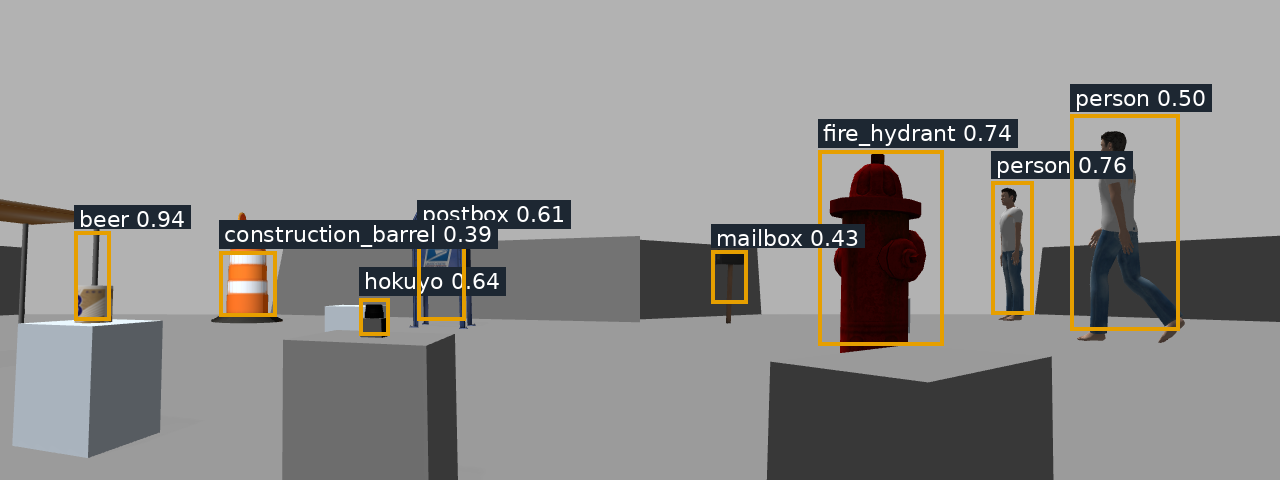
\includegraphics[width=0.94\textwidth]{figures/yolo_final_world_detection.png}
\caption{Two newly captured TurtleBot3 RGB views in the final 26-target world. Boxes, labels, and displayed confidences are actual outputs of the principal YOLO11n checkpoint used in all 51 trials, at inference threshold 0.25. Capture and annotation occurred outside the recorded trials; this figure shows 2-D inference, not depth validation, instance matching, or a trial outcome.}
\label{fig:yolo}
\end{figure*}

The deployed detector checkpoint was fine-tuned for 10 epochs at 640-pixel image size. This paper reports discovery only for the 26 target instances in the final world. A detector-only precision or mAP measurement for exactly this 26-target evaluation was not saved, so no such statistic is claimed.

\subsection{Unique-Object Scoring}
A detection needs a valid world position and must exceed its class threshold. Observations of the same class within 0.75\,m form a cluster; a cluster requires at least two distinct frame stamps. Confirmed clusters are matched one-to-one to same-class SDF instances within 1.25\,m planar error. Class aliases combine two person models under \texttt{person} and map the point-cloud bottle/doll to detector classes. Duplicates cannot count twice for an instance. The evaluator reads known SDF target poses for \emph{scoring}; policies and coverage planner do not receive them. Thus the metric is a class-and-position match, not manually verified recognition of each physical object.

\section{Problem Formulation and Controllers}
\subsection{Observation, Actions, and Reward}
The final policy environment is a partially observed discrete-action process. At step $t$, both learned models receive
\begin{equation}
s_t=[\ell_{1:360},x_t,y_t,\psi_t,c_t,\nu_{1:8}]
\in\mathbb{R}^{372},
\label{eq:state}
\end{equation}
where $\ell$ is LiDAR range clipped and scaled to 3.5\,m, $(x,y,\psi)$ is odometry pose, $c_t\in[0,1]$ is latest detection confidence (zeroed after 0.75\,s), and $\nu_{1:8}$ estimates unvisited 0.5-m cells in eight relative directions. The map planner consumes a separate SLAM occupancy grid, which is not a network input.

Actions $A=\{0,1,2\}$ are forward $(v,\omega)=(0.25,0)$, left $(0,0.90)$, and right $(0,-0.90)$ in m/s and rad/s. The evaluator advances each nominal action for 0.15\,s, though safety recovery may issue other velocities. The final environment reward is
\begin{equation}
\begin{aligned}
r_t={}&5I_{\mathrm{new\ cell}}+0.1c_t
+10n_{\mathrm{new\ cluster}}\\
&-I_{\mathrm{collision}}-0.2I_{\mathrm{revisit}}-0.02+u_t,\\
u_t={}&\begin{cases}0.05,&v_t>0,\\-0.03,&v_t\leq0.\end{cases}
\end{aligned}
\label{eq:reward}
\end{equation}
where $I$ is an indicator and $n_{\mathrm{new\ cluster}}$ counts newly confirmed \emph{local} clusters. The primary outcome instead uses separate one-to-one world matching. The Gymnasium environment returns $(s_{t+1},r_t,\mathrm{terminated},\mathrm{truncated},\mathrm{info})$. Collision is penalized but does not alone terminate an episode.

Figure~\ref{fig:loop} summarizes the feedback sequence; assistance can replace a policy proposal before robot actuation.

\begin{figure}[t]
\centering
\resizebox{\columnwidth}{!}{%
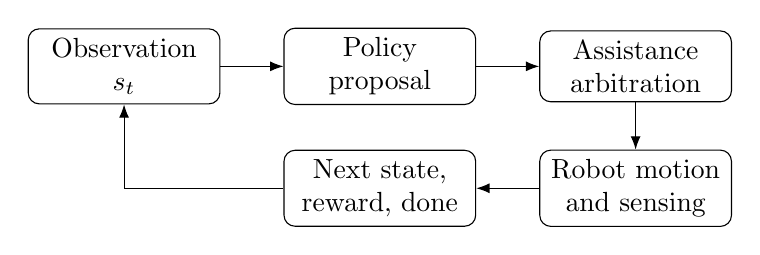
\begin{tikzpicture}[>=Latex,node distance=6mm and 8mm,
b/.style={draw,rounded corners,align=center,text width=22mm,minimum height=9mm}]
\node[b] (o) {Observation\\$s_t$};
\node[b,right=of o] (p) {Policy\\proposal};
\node[b,right=of p] (a) {Assistance\\arbitration};
\node[b,below=of a] (r) {Robot motion\\and sensing};
\node[b,left=of r] (n) {Next state,\\reward, done};
\draw[->] (o)--(p);
\draw[->] (p)--(a);
\draw[->] (a)--(r);
\draw[->] (r)--(n);
\draw[->] (n.west)-|([yshift=-6mm]o.south)--(o.south);
\end{tikzpicture}}
\caption{One interaction step. Random has no assistance override; learned policy proposals may be replaced by coverage, inspection, confirmation, or recovery actions.}
\label{fig:loop}
\end{figure}

\subsection{Double Deep Q-Network}
The project subclasses Stable-Baselines3 DQN and replaces its target calculation with Double DQN:
\begin{equation}
y_t=r_t+\gamma(1-d_t)Q_{\theta^-}
\!\left(s_{t+1},\arg\max_a Q_\theta(s_{t+1},a)\right),
\label{eq:ddqn}
\end{equation}
where $d_t$ is the terminal indicator, $\theta$ is the online network, $\theta^-$ is the target network, and $\gamma=0.99$~\cite{vanhasselt2016}. Replay-buffer samples train a two-hidden-layer, 128-unit-per-layer Q-network with smooth-$L_1$ loss. Saved-model settings are learning rate $10^{-3}$, replay capacity 50,000, batch size 64, target update interval 1,000, and final training epsilon 0.05. Evaluation uses deterministic prediction.

The checkpoint path contains the name \texttt{ddqn\_safe\_50000}, but its training summary and loaded model record \emph{34,763} steps; the run was interrupted, with 40,000 steps requested. Its training world and detector differ from the final evaluation world and detector. The filename is not evidence of 50,000 completed steps.

\subsection{Proximal Policy Optimization}
The PPO policy has separate 128--128 hidden-layer actor and critic MLPs. Its clipped surrogate objective is
\begin{equation}
\begin{aligned}
L^{\mathrm{CLIP}}(\theta)=\mathbb{E}_t\bigl[\min\bigl(
&\rho_t(\theta)\hat A_t,\\
&\operatorname{clip}(\rho_t(\theta),1-\epsilon,1+\epsilon)
\hat A_t\bigr)\bigr],
\end{aligned}
\label{eq:ppo}
\end{equation}
where $\rho_t(\theta)=\pi_\theta(a_t|s_t)/
\pi_{\theta_{\mathrm{old}}}(a_t|s_t)$, $\hat A_t$ is estimated advantage, and $\epsilon=0.2$ controls update size~\cite{schulman2017}. Saved settings are learning rate $3\times10^{-4}$, $\gamma=0.99$, GAE parameter 0.95, 250-step rollouts, batch size 50, ten optimization epochs, and zero entropy coefficient. The training record reports 10,000 steps in a different pedestal world with a different detector checkpoint. Evaluation is deterministic. The saved training episodes are not used as results for the final 26-target world.

Figure~\ref{fig:rlcompare} contrasts the updates in (\ref{eq:ddqn}) and (\ref{eq:ppo}). DDQN learns from replay and a delayed target network; PPO learns from recent rollouts with actor and critic networks.

\begin{figure*}[t]
\centering
\resizebox{0.84\textwidth}{!}{%
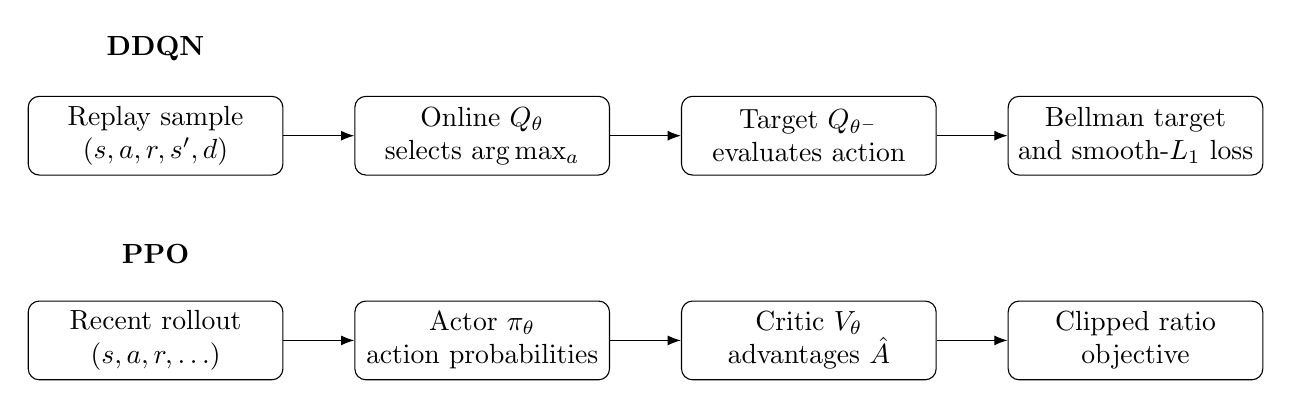
\begin{tikzpicture}[>=Latex,node distance=8mm and 9mm,
b/.style={draw,rounded corners,align=center,text width=30mm,minimum height=10mm},
head/.style={font=\bfseries}]
\node[head] at (0,1.1) {DDQN};
\node[b] (replay) at (0,0) {Replay sample\\$(s,a,r,s',d)$};
\node[b,right=of replay] (online) {Online $Q_\theta$\\selects $\arg\max_a$};
\node[b,right=of online] (target) {Target $Q_{\theta^-}$\\evaluates action};
\node[b,right=of target] (loss) {Bellman target\\and smooth-$L_1$ loss};
\draw[->] (replay)--(online);
\draw[->] (online)--(target);
\draw[->] (target)--(loss);
\node[head] at (0,-1.5) {PPO};
\node[b] (roll) at (0,-2.6) {Recent rollout\\$(s,a,r,\ldots)$};
\node[b,right=of roll] (actor) {Actor $\pi_\theta$\\action probabilities};
\node[b,right=of actor] (critic) {Critic $V_\theta$\\advantages $\hat A$};
\node[b,right=of critic] (clip) {Clipped ratio\\objective};
\draw[->] (roll)--(actor);
\draw[->] (actor)--(critic);
\draw[->] (critic)--(clip);
\end{tikzpicture}}
\caption{Implementation-level update distinction. DDQN uses replay and online/target Q networks; PPO uses recent rollouts and separate actor/critic MLPs. Both are later evaluated as deterministic saved policies.}
\label{fig:rlcompare}
\end{figure*}

\subsection{Random Actions and Coverage Assistance}
The Random baseline samples uniformly from the same three nominal actions using its trial seed. It uses the same environment, detector stack, target inventory, and action duration, but has no global coverage planner, inspection sweep, detection-confirmation turns, or safety-recovery wrapper.

For DDQN and PPO, \texttt{GlobalCoverageAssist} subscribes to the SLAM occupancy grid \texttt{/map}, transforms visits to map coordinates, and steers toward reachable unvisited frontiers after one second without a new cell. It also supports breadcrumb return and LiDAR-based escape. Assisted runs perform 1-m-spaced inspection sweeps, turn to confirm emerging detections, and recover from stalls. These routines can override policy actions. They do not use evaluator target coordinates, but they materially alter control and are part of the evaluated treatment. Every step logs the policy proposal, applied action, and top-level action source.

\section{Experimental Design}
\subsection{Final Evaluation Protocol}
All 51 final runs use \texttt{spaced\_objects\_reliable\_26\_v4.world}, the same principal balanced YOLO checkpoint, start pose, target definition, and a 12-minute maximum. Each method has 17 records, seeds 42--58. A run stops at 26 matched instances or the wall-clock deadline; startup precedes the timed loop. World matching has the same 1.25-m tolerance. Thresholds relevant to the 26 targets are shared by all series: base 0.25, bottle/doll 0.20, and gear part 0.15. Table~\ref{tab:setup} summarizes configuration.

The three original series are \texttt{ddqn\_26\_17\_20261120}, \texttt{ppo\_26\_17\_20261121}, and \texttt{random\_26\_17\_20261122} under \texttt{rl\_evaluations/}. Each of the 51 CSV rows was cross-checked against its unique per-run \texttt{summary.json} and \texttt{world\_coverage\_report.json}. All rows had target count 26 and the indicated world/model; all recorded \texttt{guided\_completion\_enabled=false}. Only these final 26-instance runs are analyzed.

\begin{table}[t]
\caption{Final evaluation configuration}
\label{tab:setup}
\centering\footnotesize
\begin{tabular}{@{}p{0.30\columnwidth}p{0.64\columnwidth}@{}}
\toprule
Setting & Value\\ \midrule
Robot and middleware & Simulated TurtleBot3 Burger; ROS 2 Humble; Gazebo 11.10.2\\
World and targets & 18\,m $\times$ 18\,m bounded SDF; 26 included instances\\
Sensors & 360-beam LiDAR, RGB--depth camera, odometry\\
Detector & Fine-tuned YOLO11n plus person and bottle/doll fallback models\\
Policy interface & 372-dimensional state, three discrete actions\\
Trials and seeds & 17 per method; seeds 42--58\\
Stop & 12 min or 26 matched world instances\\
DDQN/PPO control & Saved deterministic policy plus SLAM coverage, inspection, confirmation, safety recovery\\
Random control & Uniform action sampling without these assistance routines\\
\bottomrule
\end{tabular}
\end{table}

\subsection{Metrics and Uncertainty}
For trial $i$, let $N_i$ be matched instances, $T_i$ elapsed wall-clock minutes, and $F_i=I(N_i=26)$. We compute
\begin{equation}
C_i=100N_i/26,\quad
\bar N=\frac{1}{17}\sum_{i=1}^{17}N_i,\quad
S=\frac{100}{17}\sum_{i=1}^{17}F_i.
\label{eq:metrics}
\end{equation}
Successful completion time is
$\bar T_{\rm complete}=\sum_i F_iT_i/\sum_i F_i$; mean elapsed duration is $17^{-1}\sum_iT_i$ and includes timeouts. These are different estimands. We report sample standard deviation (SD) for counts and 95\% Wilson intervals~\cite{wilson1927} for completion proportions. A cumulative completion plot retains unsuccessful runs as right-censored at their time limit. The small sample and assistance imbalance argue against a causal algorithm ranking. Reward is descriptive only: overridden actions and different training conditions limit its comparability.

\section{Results}
\subsection{Per-Trial Object Coverage}
Table~\ref{tab:trials} contains all 51 final result rows as matched counts and elapsed times; Fig.~\ref{fig:trials} shows the counts. The random configuration reached 8/26 in trials 8 and 11, illustrating larger across-seed variability than the two assisted configurations. Timed-out trials remain in all analyses and are never imputed as successful completions.

\begin{table*}[!t]
\caption{All 51 final trials. Each method has matched objects $N$ and elapsed minutes $T$. A time near 12 min with $N<26$ is a timeout. Trial number corresponds to the same nominal seed across methods.}
\label{tab:trials}
\centering\footnotesize
\begin{tabular}{@{}cc rr rr rr@{}}
\toprule
& & \multicolumn{2}{c}{DDQN + assistance} & \multicolumn{2}{c}{PPO + assistance} & \multicolumn{2}{c}{Random only}\\
Trial & Seed & $N$ & $T$ & $N$ & $T$ & $N$ & $T$\\ \midrule
1 & 42 & 26 & 2.90 & 26 & 1.77 & 23 & 12.00\\
2 & 43 & 26 & 3.29 & 22 & 12.00 & 21 & 12.00\\
3 & 44 & 26 & 3.76 & 26 & 2.55 & 22 & 12.00\\
4 & 45 & 26 & 6.53 & 26 & 1.86 & 26 & 6.95\\
5 & 46 & 24 & 12.00 & 26 & 5.49 & 12 & 12.00\\
6 & 47 & 25 & 12.00 & 26 & 3.95 & 20 & 12.00\\
7 & 48 & 23 & 12.00 & 25 & 12.00 & 25 & 12.00\\
8 & 49 & 26 & 1.69 & 23 & 12.00 & 8 & 12.00\\
9 & 50 & 25 & 12.00 & 26 & 3.19 & 24 & 12.00\\
10 & 51 & 26 & 1.85 & 25 & 12.00 & 18 & 12.00\\
11 & 52 & 26 & 1.97 & 25 & 12.00 & 8 & 12.00\\
12 & 53 & 26 & 4.36 & 26 & 2.08 & 25 & 12.00\\
13 & 54 & 25 & 12.00 & 25 & 12.00 & 19 & 12.00\\
14 & 55 & 26 & 2.66 & 26 & 3.03 & 16 & 12.00\\
15 & 56 & 26 & 2.09 & 25 & 12.00 & 22 & 12.00\\
16 & 57 & 26 & 2.11 & 26 & 3.50 & 19 & 12.00\\
17 & 58 & 24 & 12.00 & 25 & 12.00 & 21 & 12.00\\
\bottomrule
\end{tabular}
\end{table*}

\begin{figure*}[!t]
\centering
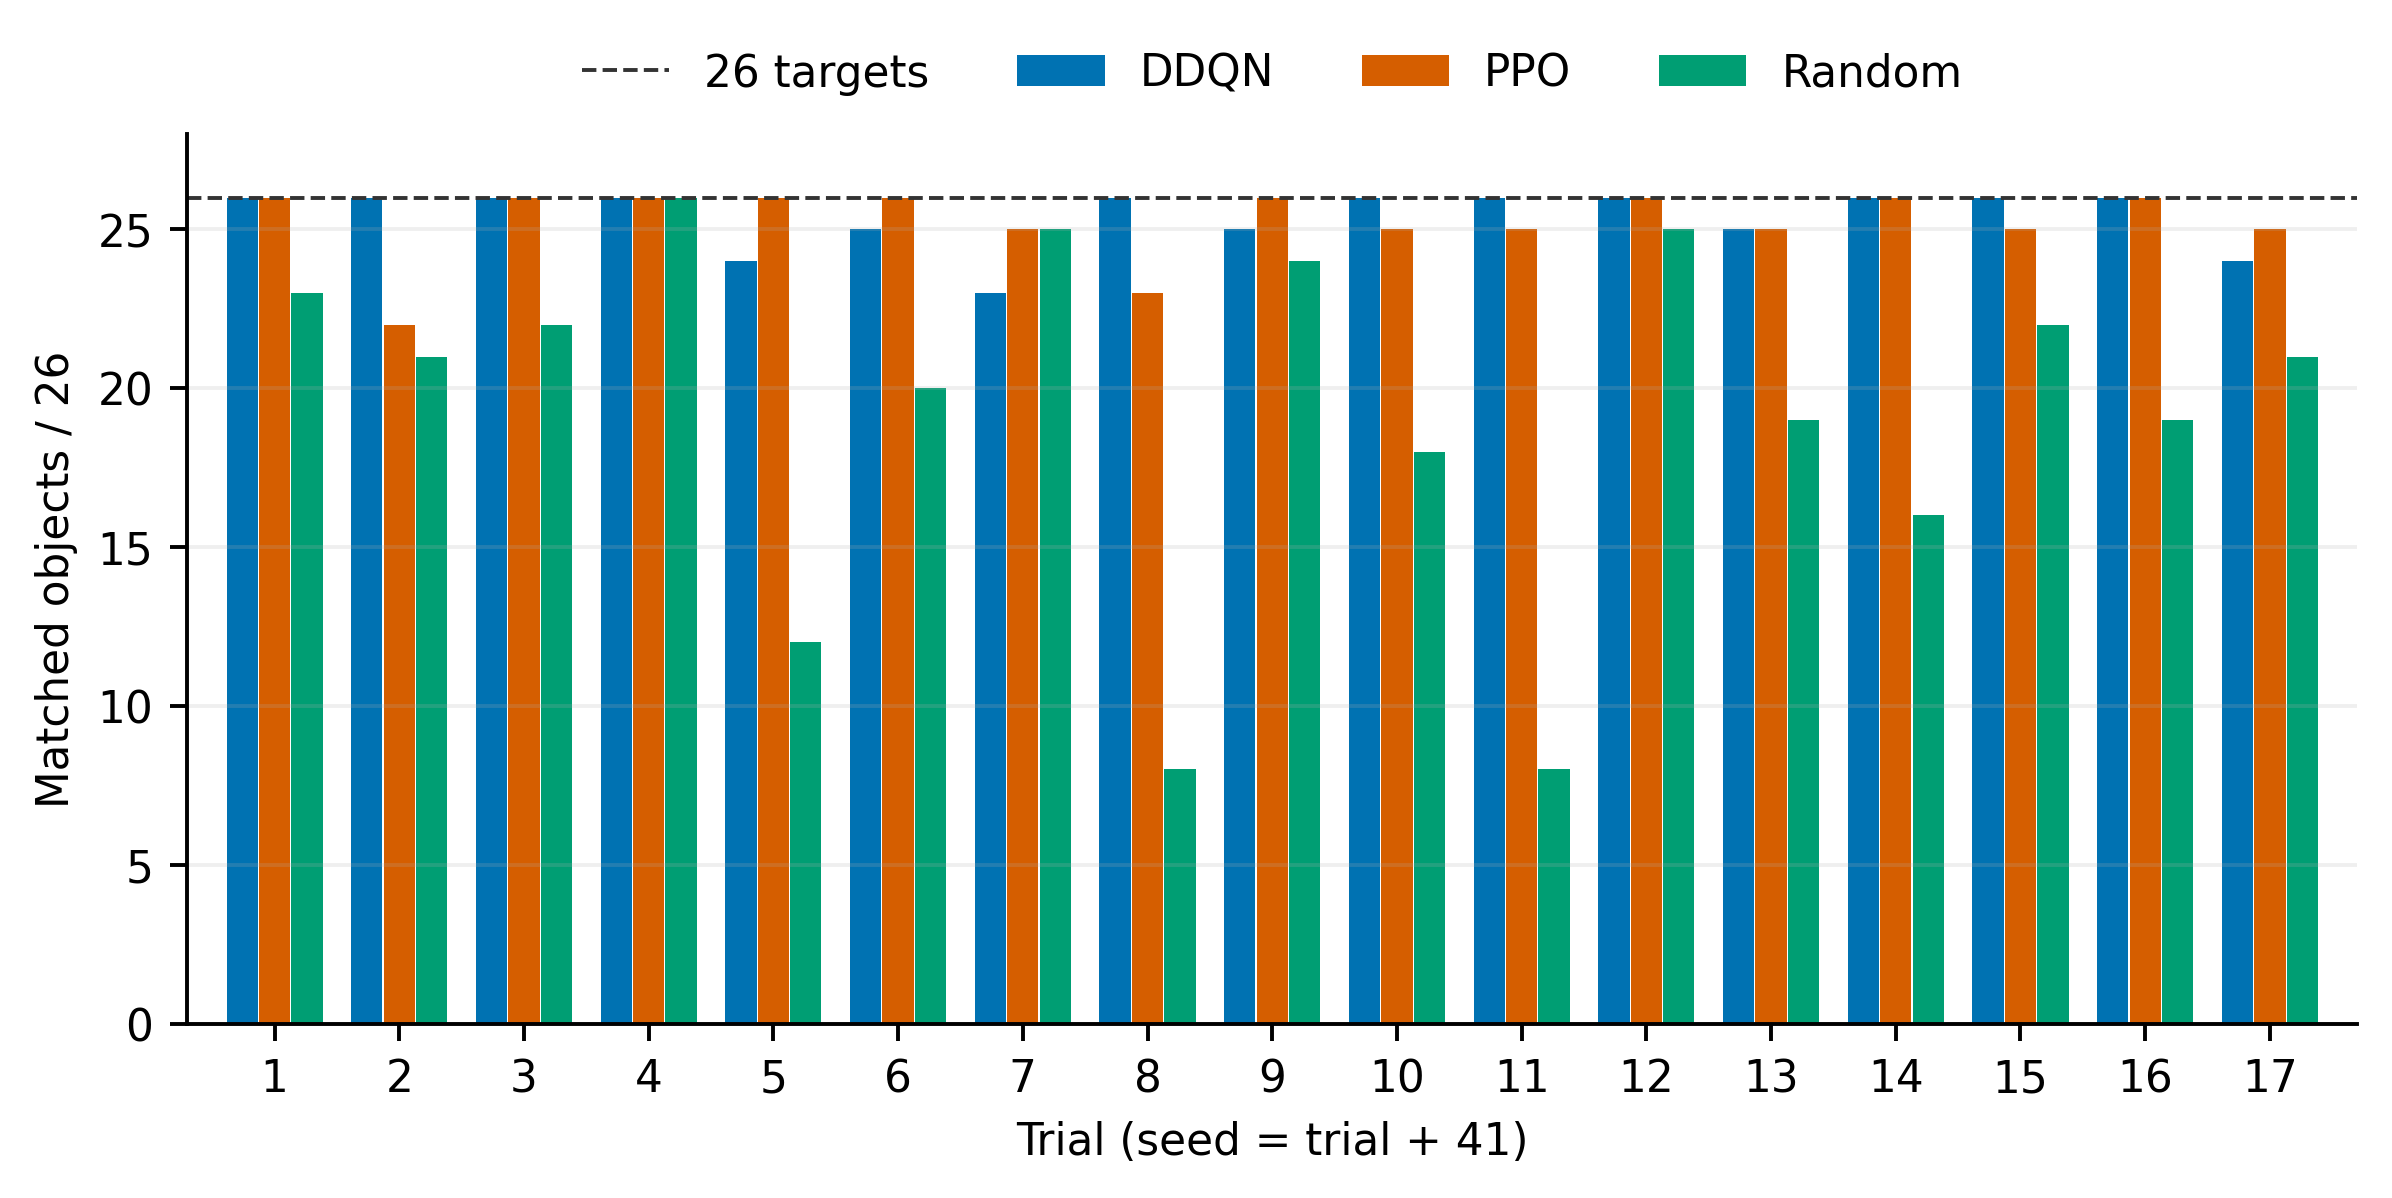
\includegraphics[width=0.84\textwidth]{figures/trial_comparison.png}
\caption{Matched target instances in each of 17 trials, calculated from per-run records. The dashed line marks complete 26/26 discovery.}
\label{fig:trials}
\end{figure*}

\subsection{Aggregate Coverage and Completion}
Table~\ref{tab:aggregate} gives independently recomputed summaries. DDQN and PPO configurations matched almost all instances on average (97.74\% and 97.06\% coverage), versus 74.43\% for Random. DDQN's mean exceeds PPO's by 0.18 object, small relative to their trial variability. Figure~\ref{fig:mean} shows individual counts and sample-SD bars. Full-discovery proportions were 64.7\%, 52.9\%, and 5.9\% (Fig.~\ref{fig:success}); 95\% Wilson intervals are wide: 41.3--82.7\%, 31.0--73.8\%, and 1.0--27.0\%. These quantify uncertainty under the evaluated configurations, not policy-only effects.

\begin{table}[!tbp]
\caption{Recomputed final-series summaries; SD is sample standard deviation}
\label{tab:aggregate}
\centering\footnotesize
\begin{tabular}{@{}lrrr@{}}
\toprule
Metric & DDQN & PPO & Random\\ \midrule
Trials & 17 & 17 & 17\\
Mean matches & 25.41 & 25.24 & 19.35\\
SD of matches & 0.94 & 1.15 & 5.52\\
Median matches & 26 & 26 & 21\\
Min--max matches & 23--26 & 22--26 & 8--26\\
Mean coverage (\%) & 97.74 & 97.06 & 74.43\\
Full completions & 11 & 9 & 1\\
Mean elapsed (min) & 6.19 & 7.26 & 11.70\\
Mean successful time (min) & 3.02 & 3.05 & 6.94\\
Mean cumulative reward & $-220.29$ & $-321.18$ & $-1231.84$\\
\bottomrule
\end{tabular}
\end{table}

\begin{figure}[!tbp]
\centering
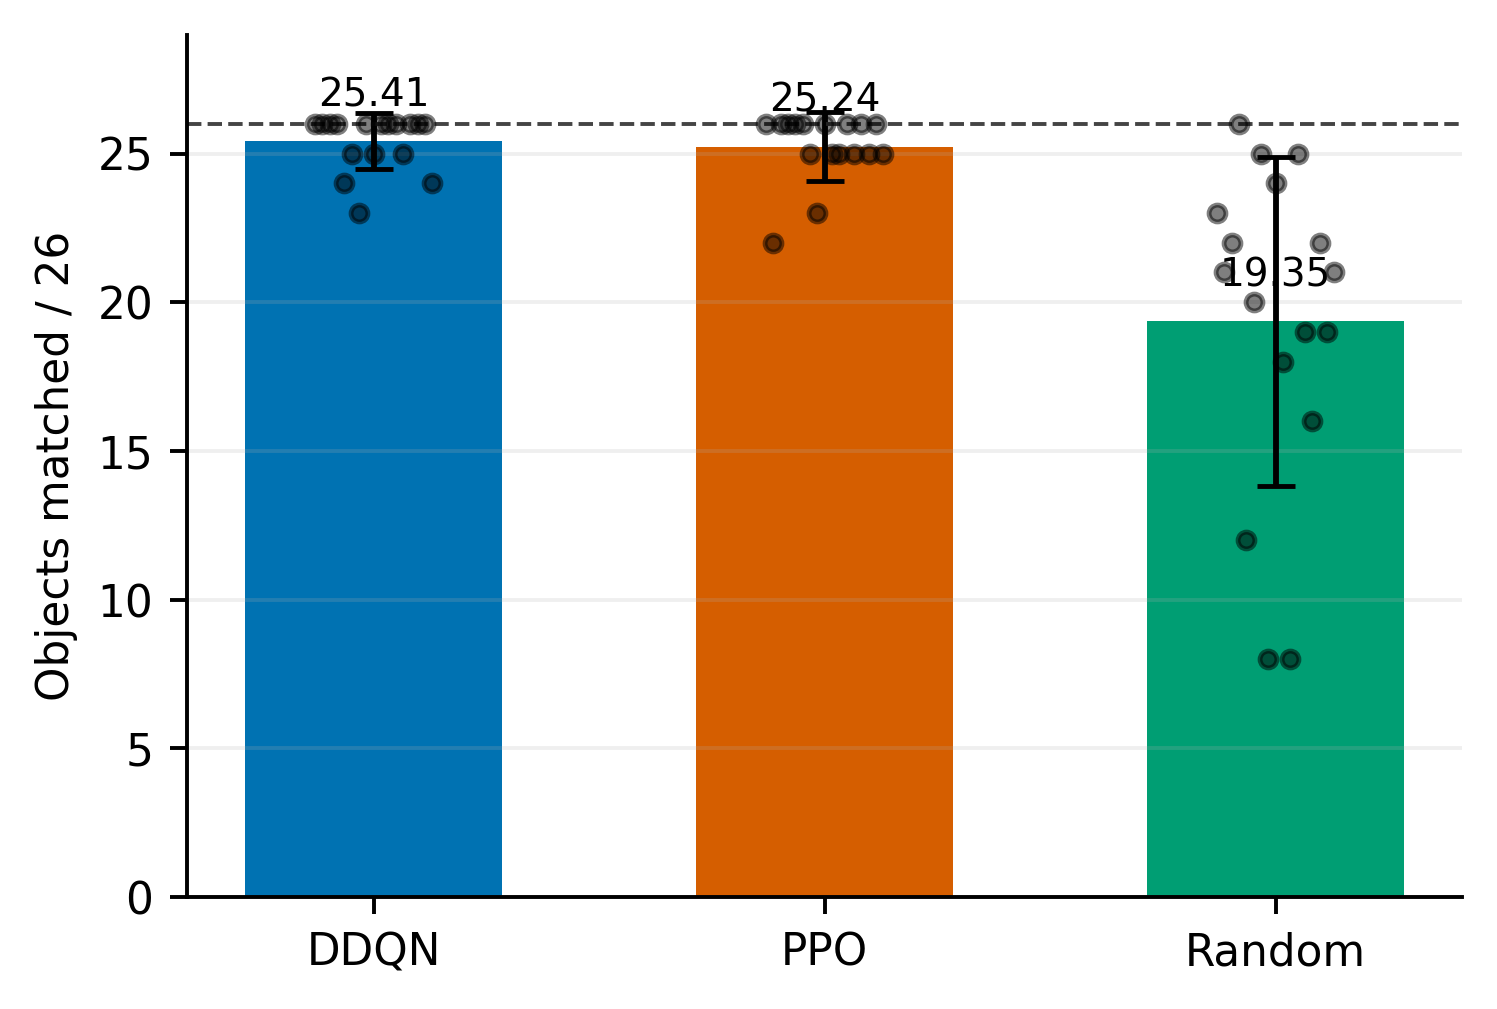
\includegraphics[width=\columnwidth]{figures/average_objects_detected.png}
\caption{Mean matched objects, individual observations, and $\pm1$ sample SD. The dashed line is the 26-object maximum. SD is variability, not a confidence interval.}
\label{fig:mean}
\end{figure}

\begin{figure}[!tbp]
\centering
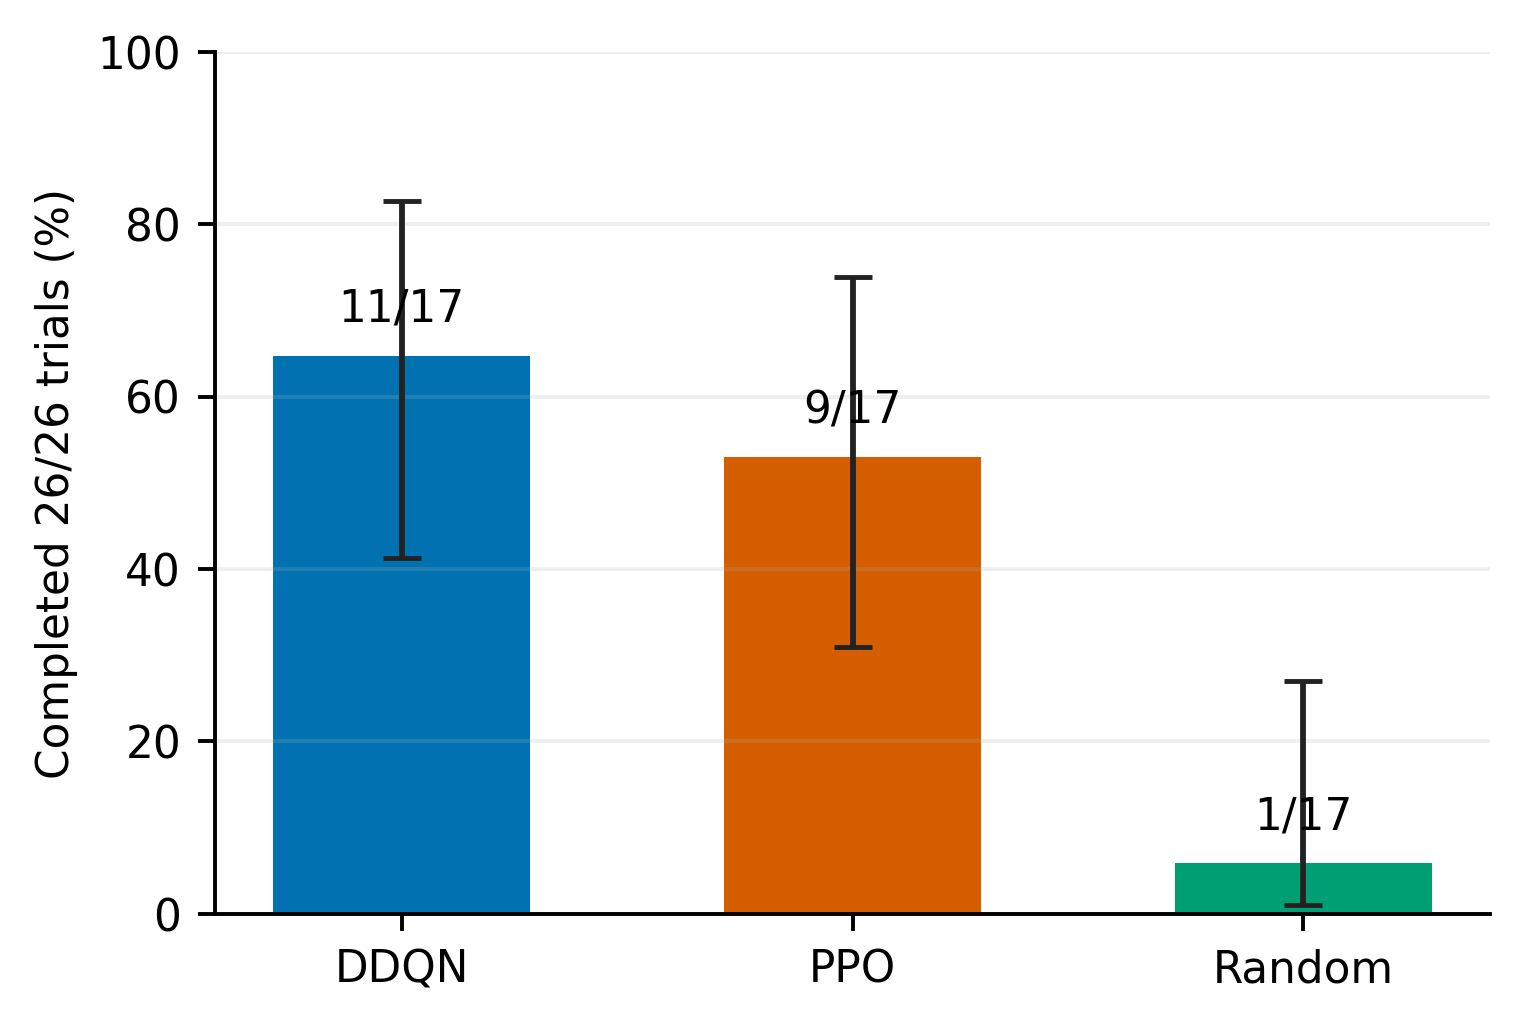
\includegraphics[width=\columnwidth]{figures/completion_success_rate.png}
\caption{Full-discovery frequency, with successful-trial counts and 95\% Wilson intervals for each $n=17$ configuration.}
\label{fig:success}
\end{figure}

\subsection{Exploration and Completion Time}
Among successful runs, mean time to the final match was 3.019\,min for DDQN, 3.046\,min for PPO, and 6.944\,min for Random; the latter estimate has only one observation (Fig.~\ref{fig:times}). Mean duration across \emph{all} runs was 6.190, 7.261, and 11.704\,min because incomplete runs continued to the deadline. Figure~\ref{fig:completion} retains unsuccessful runs as censored observations and displays the fraction completed by each time. Figure~\ref{fig:discovery} uses each object's saved confirmation timestamp to compute median cumulative matched counts across all 17 runs per method, without interpolating fictitious detections.

\begin{figure}[!tbp]
\centering
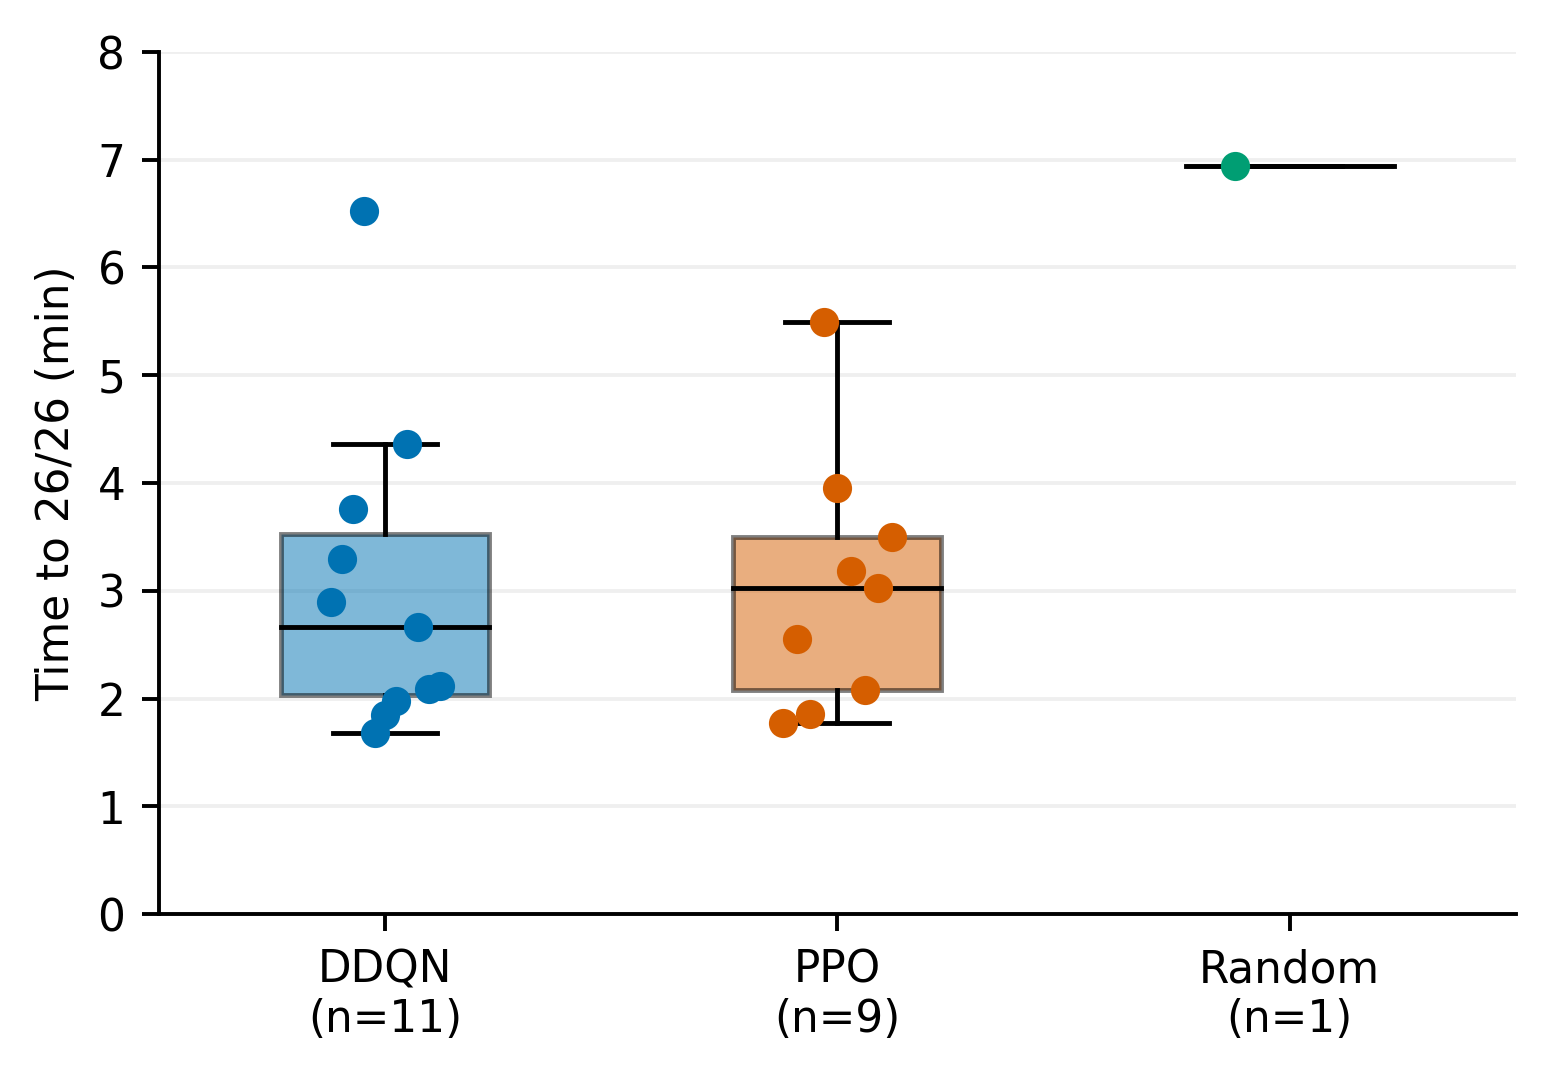
\includegraphics[width=\columnwidth]{figures/completion_time_comparison.png}
\caption{Completion times \emph{only among successful trials}; points are actual runs, boxes show quartiles, and $n$ is shown for each method. Timed-out runs are excluded here.}
\label{fig:times}
\end{figure}

\begin{figure}[!tbp]
\centering
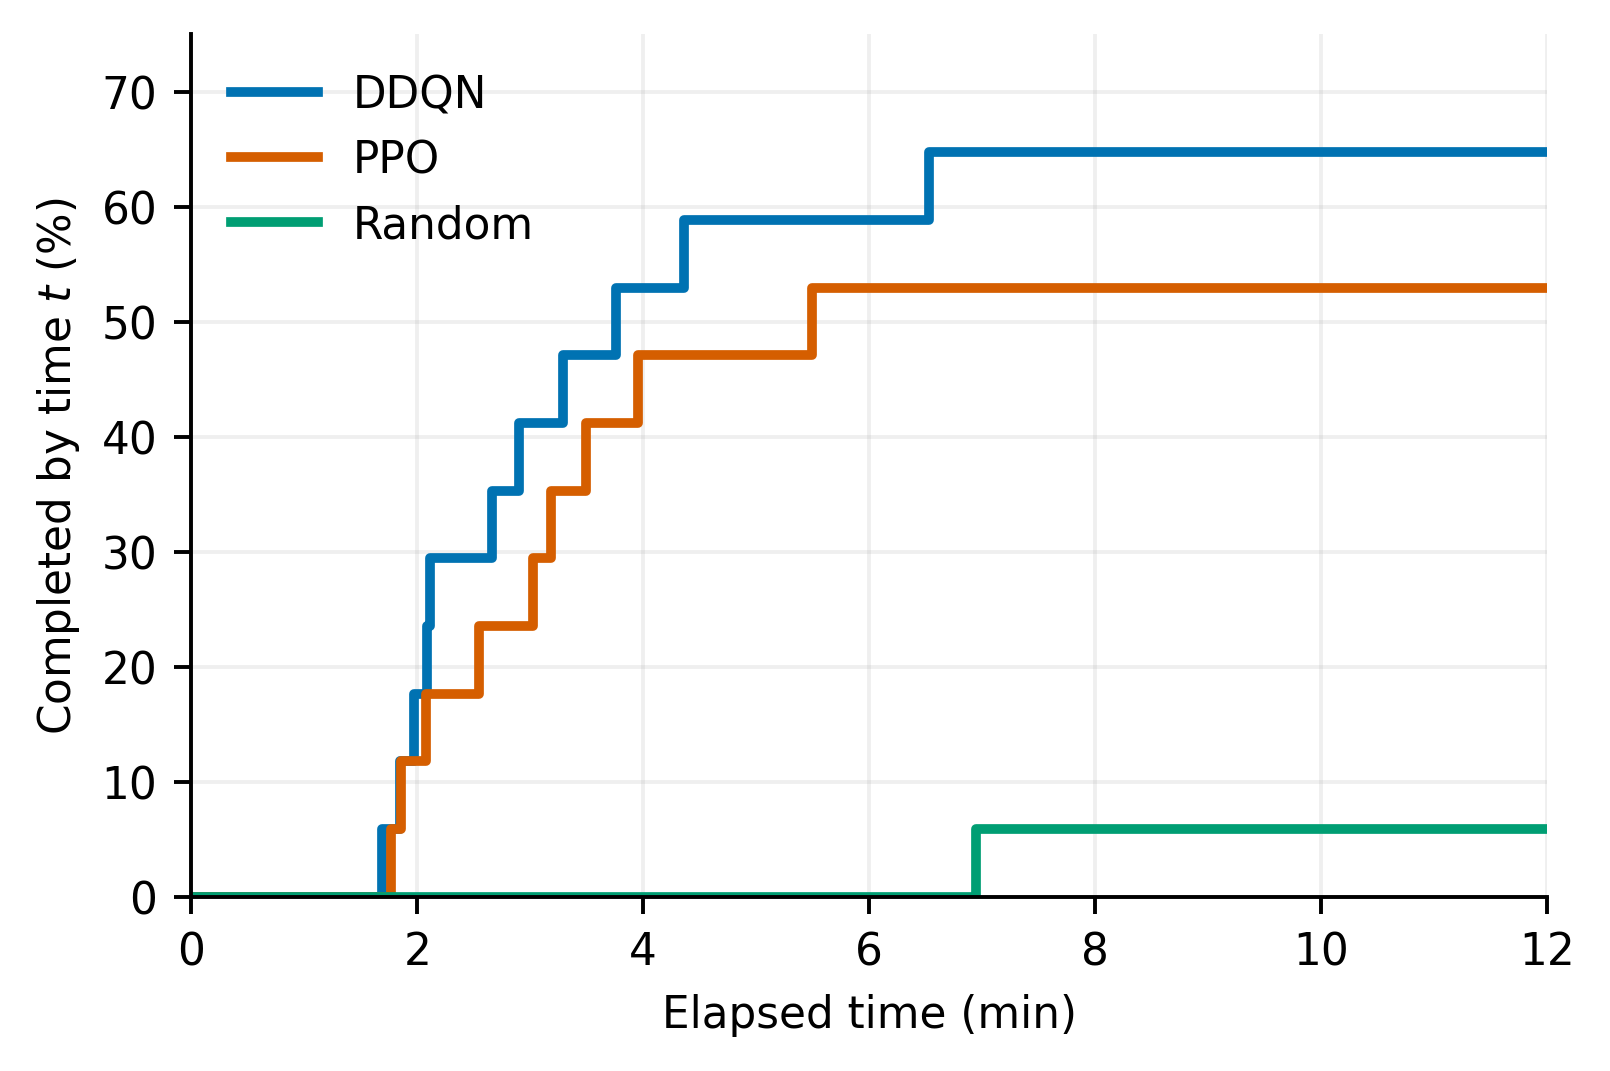
\includegraphics[width=\columnwidth]{figures/completion_cumulative.png}
\caption{Fraction reaching 26/26 by elapsed time. All 17 runs per method contribute; unfinished runs are right-censored at their observed time limits.}
\label{fig:completion}
\end{figure}

\begin{figure}[!tbp]
\centering
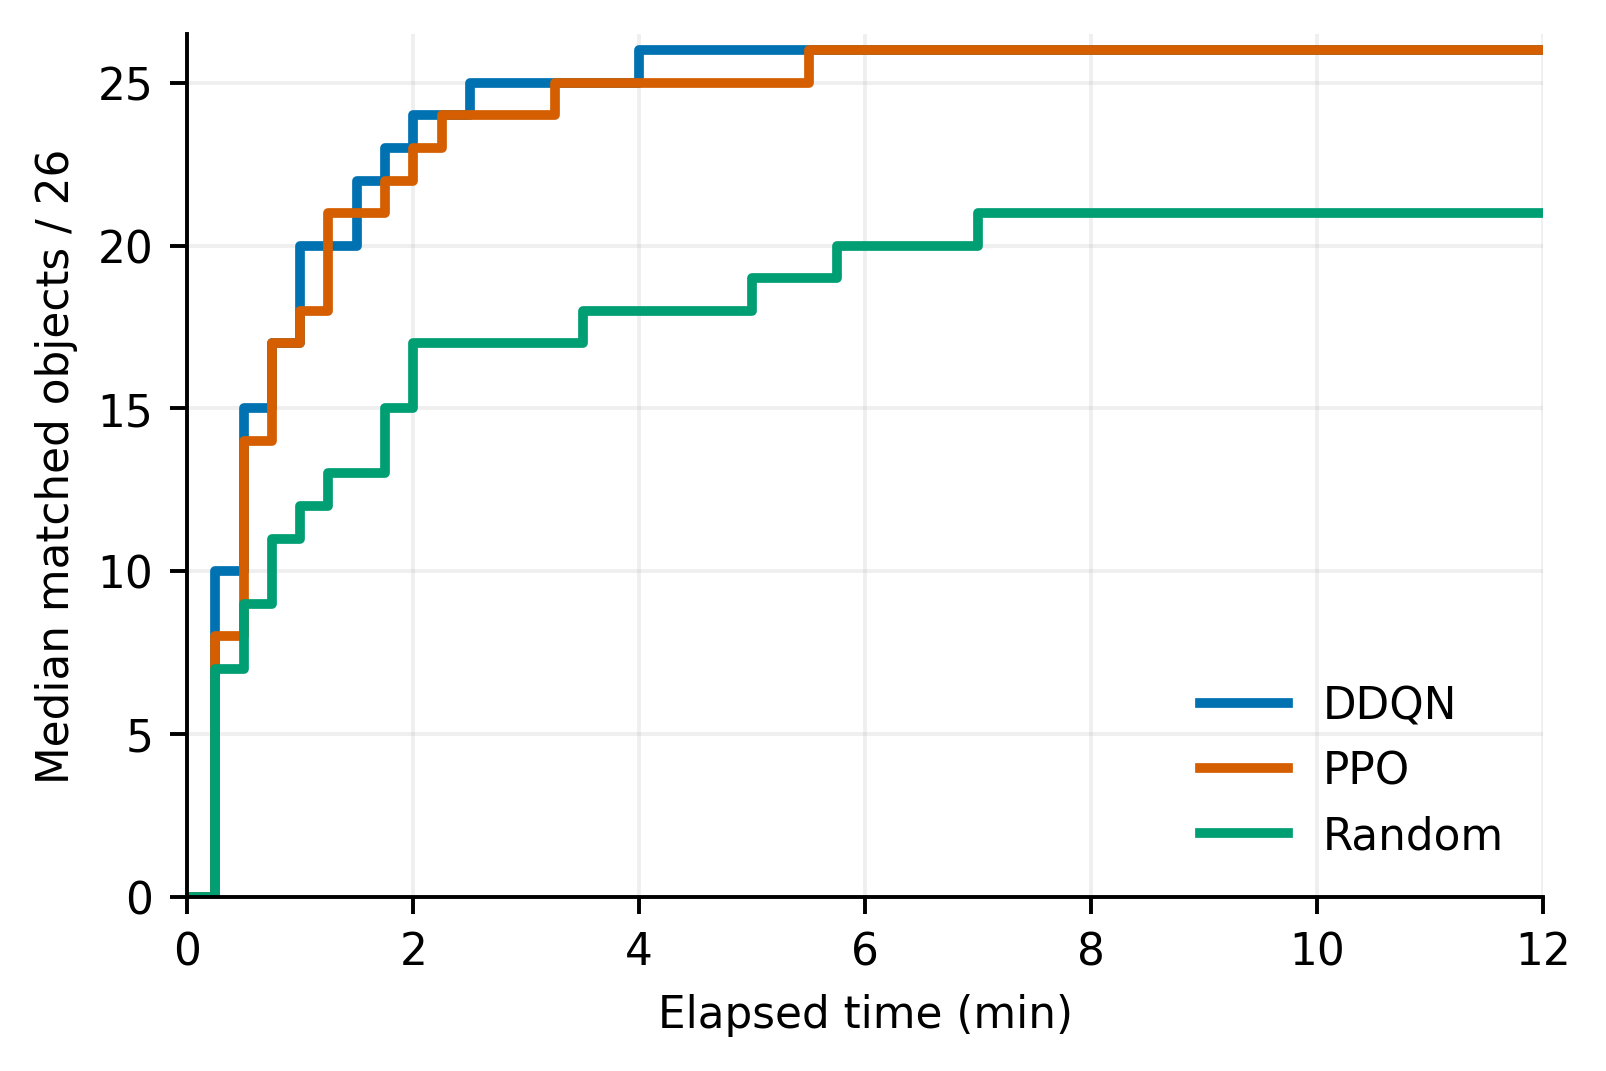
\includegraphics[width=\columnwidth]{figures/discovery_over_time.png}
\caption{Median trial-level cumulative matched instances, calculated from saved confirmation times. Counts remain fixed after each trial ends.}
\label{fig:discovery}
\end{figure}

\subsection{Applied Actions and Object-Level Results}
The action logs give the strongest interpretation check. Of 41,002 DDQN steps, 1,383 (3.4\%) applied the policy action directly, 23,655 (57.7\%) came from global coverage, 11,082 (27.0\%) from detection confirmation, and 4,882 (11.9\%) from inspection sweeps. PPO's corresponding shares over 47,972 steps were 3.3\%, 60.1\%, 23.8\%, and 12.8\%; all 78,942 random steps were logged as policy actions (Fig.~\ref{fig:control}). The category records the top-level source; safety recovery can additionally change velocity within a step. Thus the assisted configurations' apparent advantage over Random cannot be assigned to their neural policies alone.

Figure~\ref{fig:objectfreq} shows per-instance matching frequency. The grey tote and monkey wrench were each missed in two DDQN trials; lamp post, grey tote, and monkey wrench were each missed in three PPO trials. Random missed the grey tote in nine trials and the cricket ball and Hokuyo in eight each. These are world-match frequencies, not per-class detector recall. Figure~\ref{fig:traj} shows the common seed-42 trajectories, selected by seed rather than outcome. Assisted runs matched all 26 while remaining near the start; Random travelled farther but timed out at 23/26. This is consistent with wide-area visual observation and repeated turning. A match does not require physical approach to a target.

\begin{figure*}[!t]
\centering
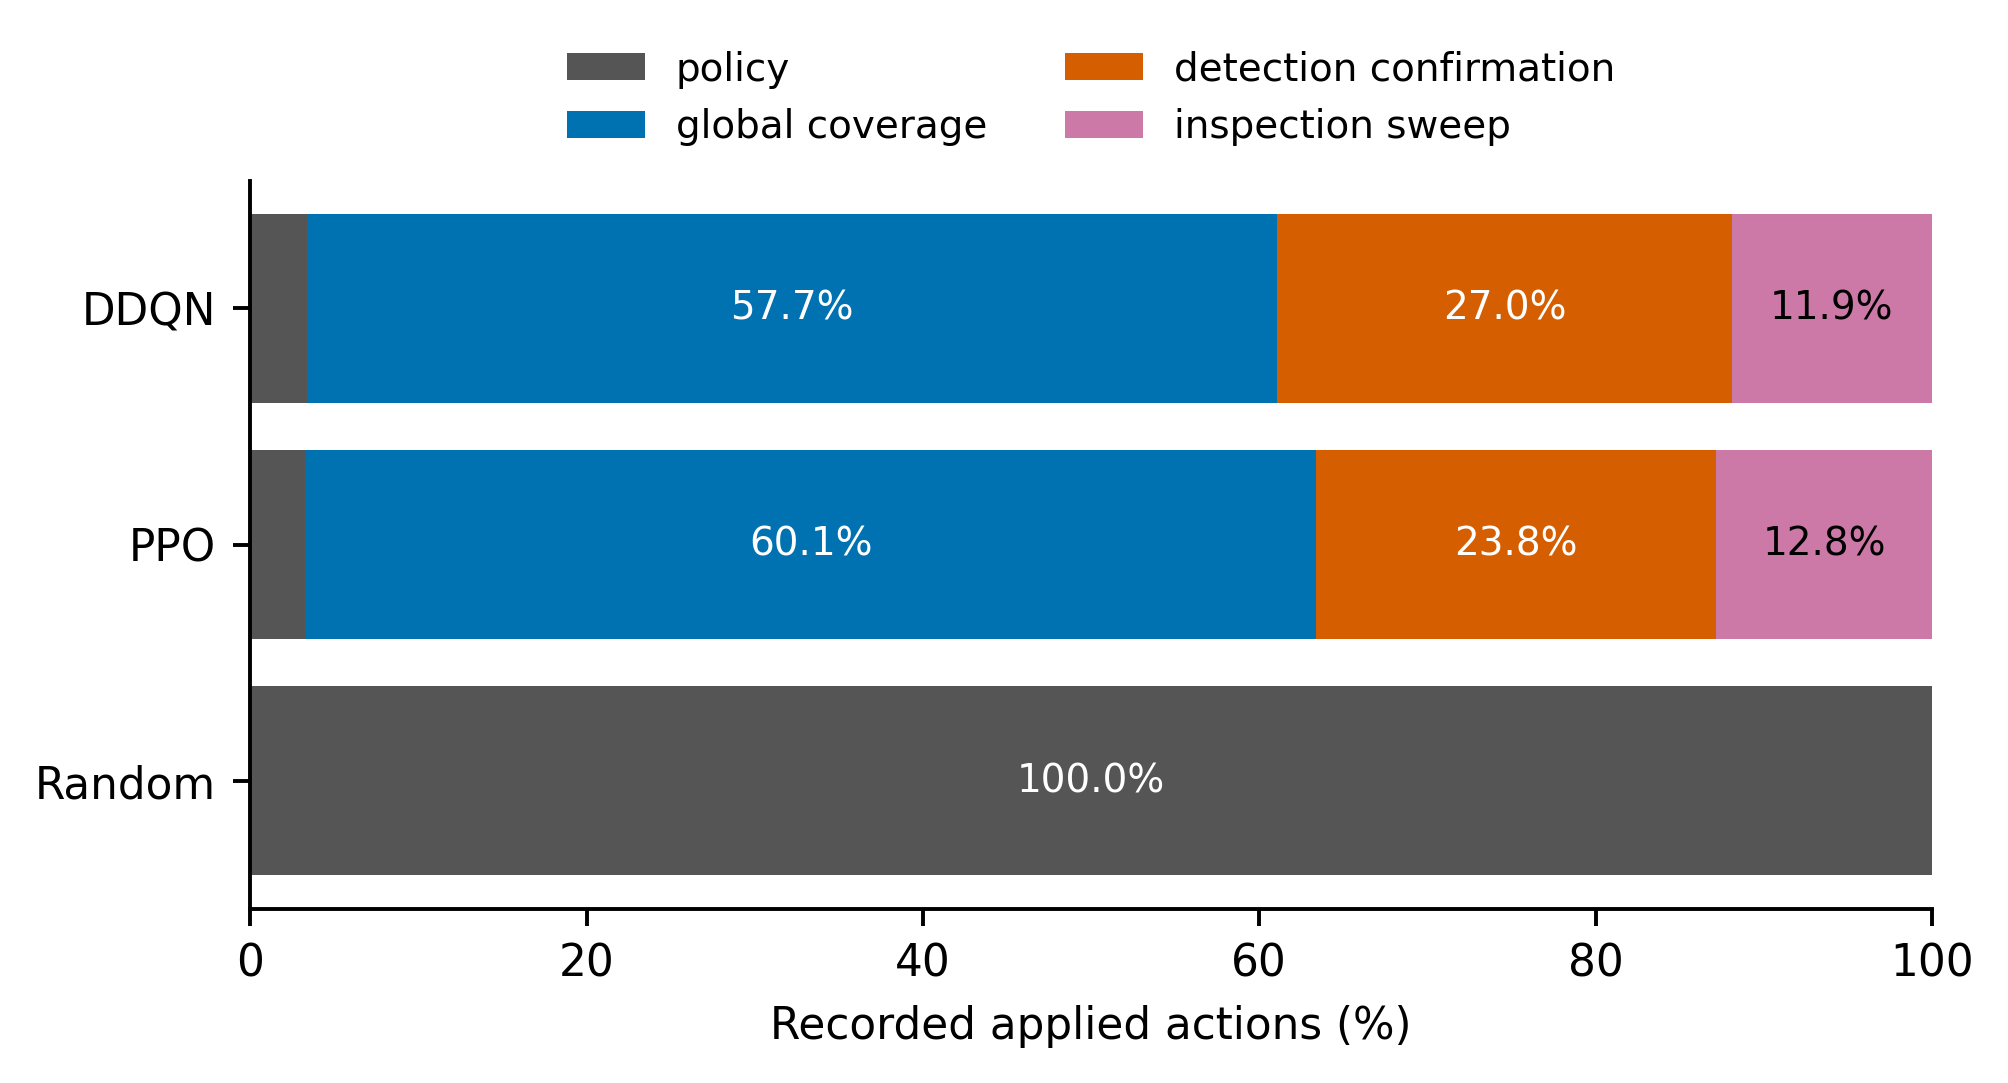
\includegraphics[width=0.74\textwidth]{figures/control_sources.png}
\caption{Applied-action sources aggregated across all \texttt{visit\_history.csv} records. Only about 3\% of learned-configuration steps directly applied the saved policy action.}
\label{fig:control}
\end{figure*}

\begin{figure*}[!t]
\centering
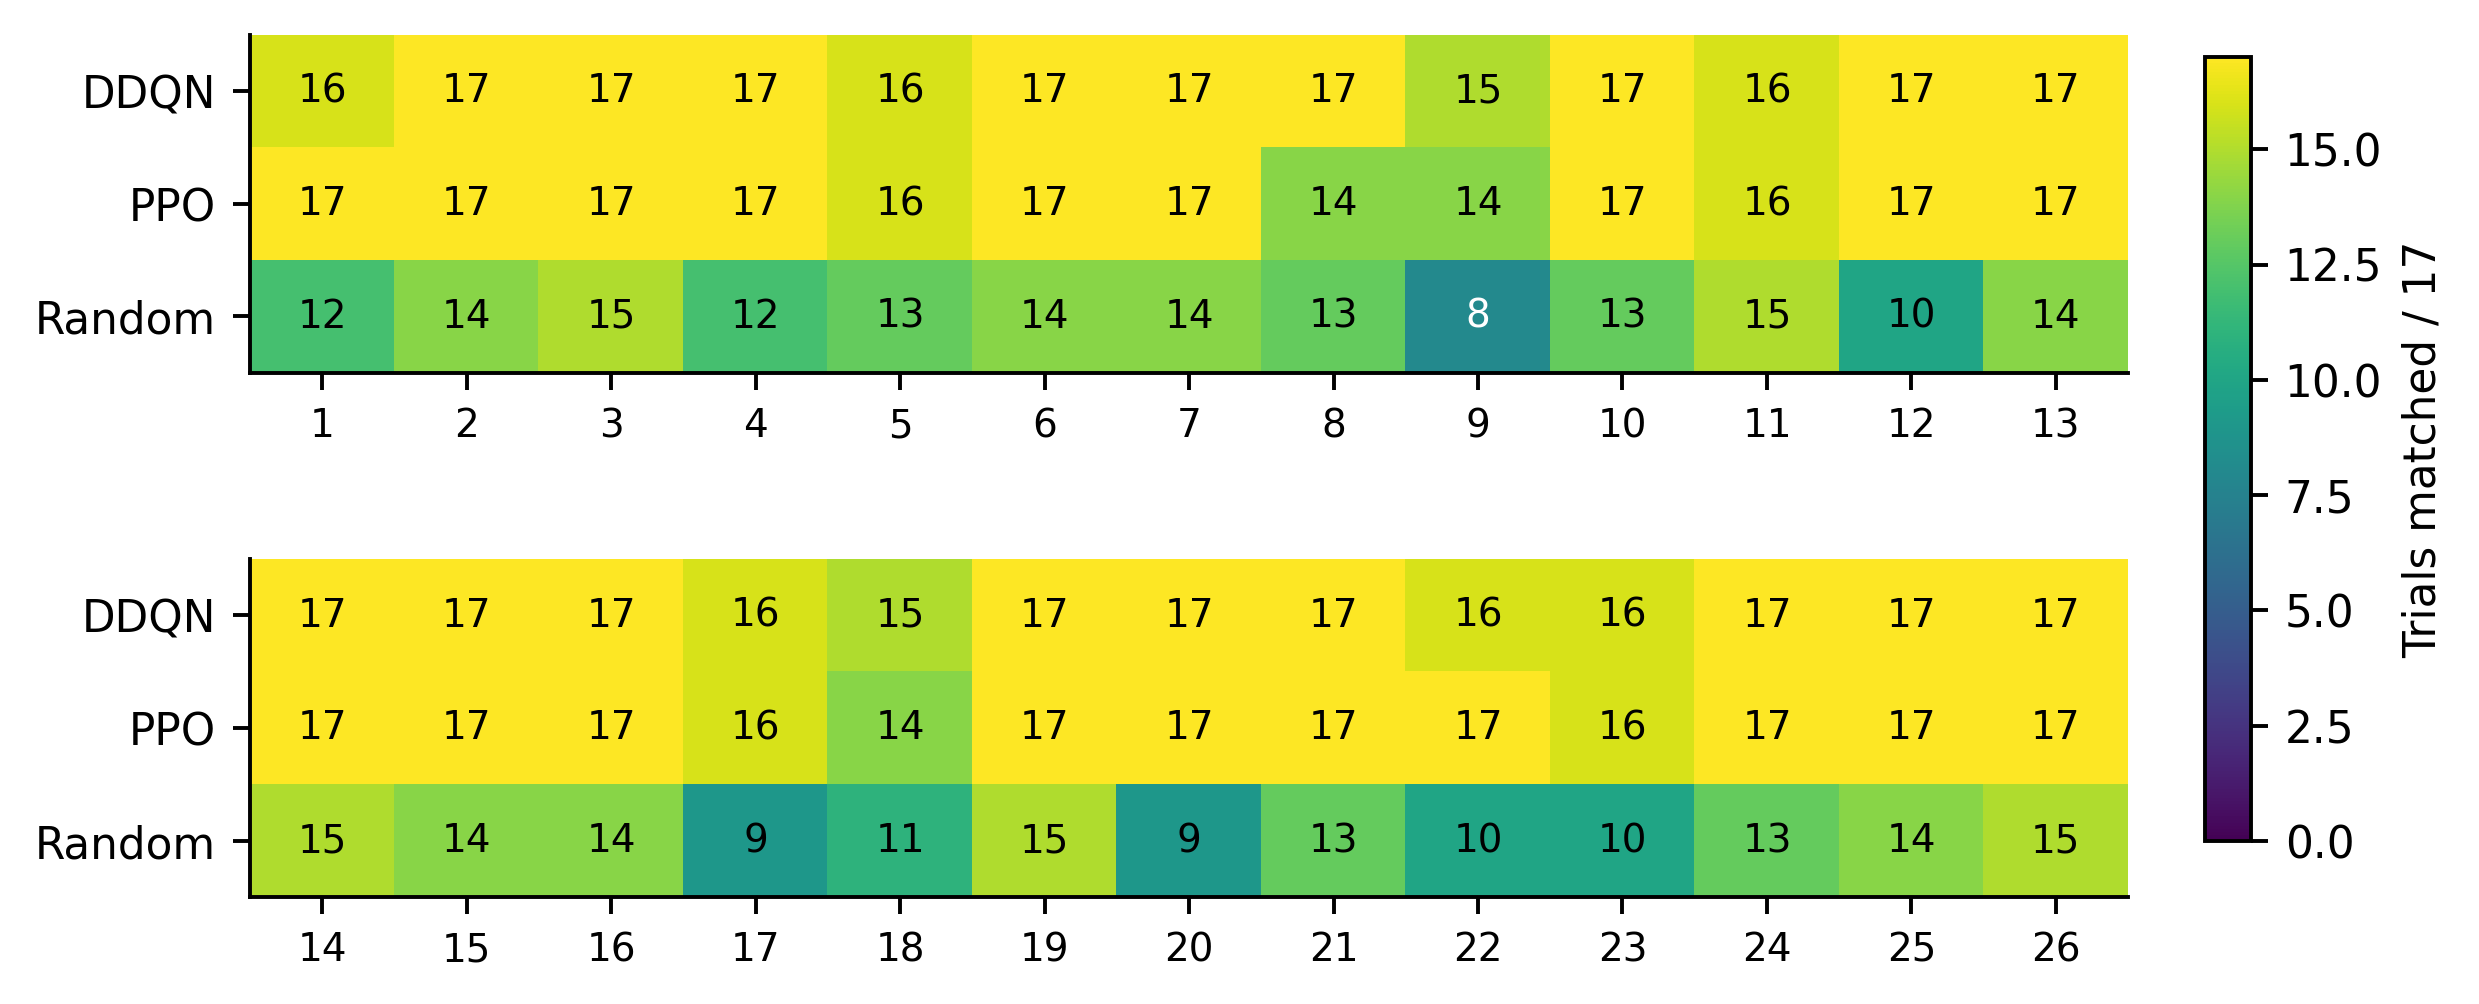
\includegraphics[width=0.92\textwidth]{figures/object_frequency.png}
\caption{Per-instance frequency of world matches out of 17 trials per method. Target IDs correspond to Table~\ref{tab:inventory}; person instances and point-cloud bottle/doll instances are counted separately.}
\label{fig:objectfreq}
\end{figure*}

\begin{figure*}[!t]
\centering
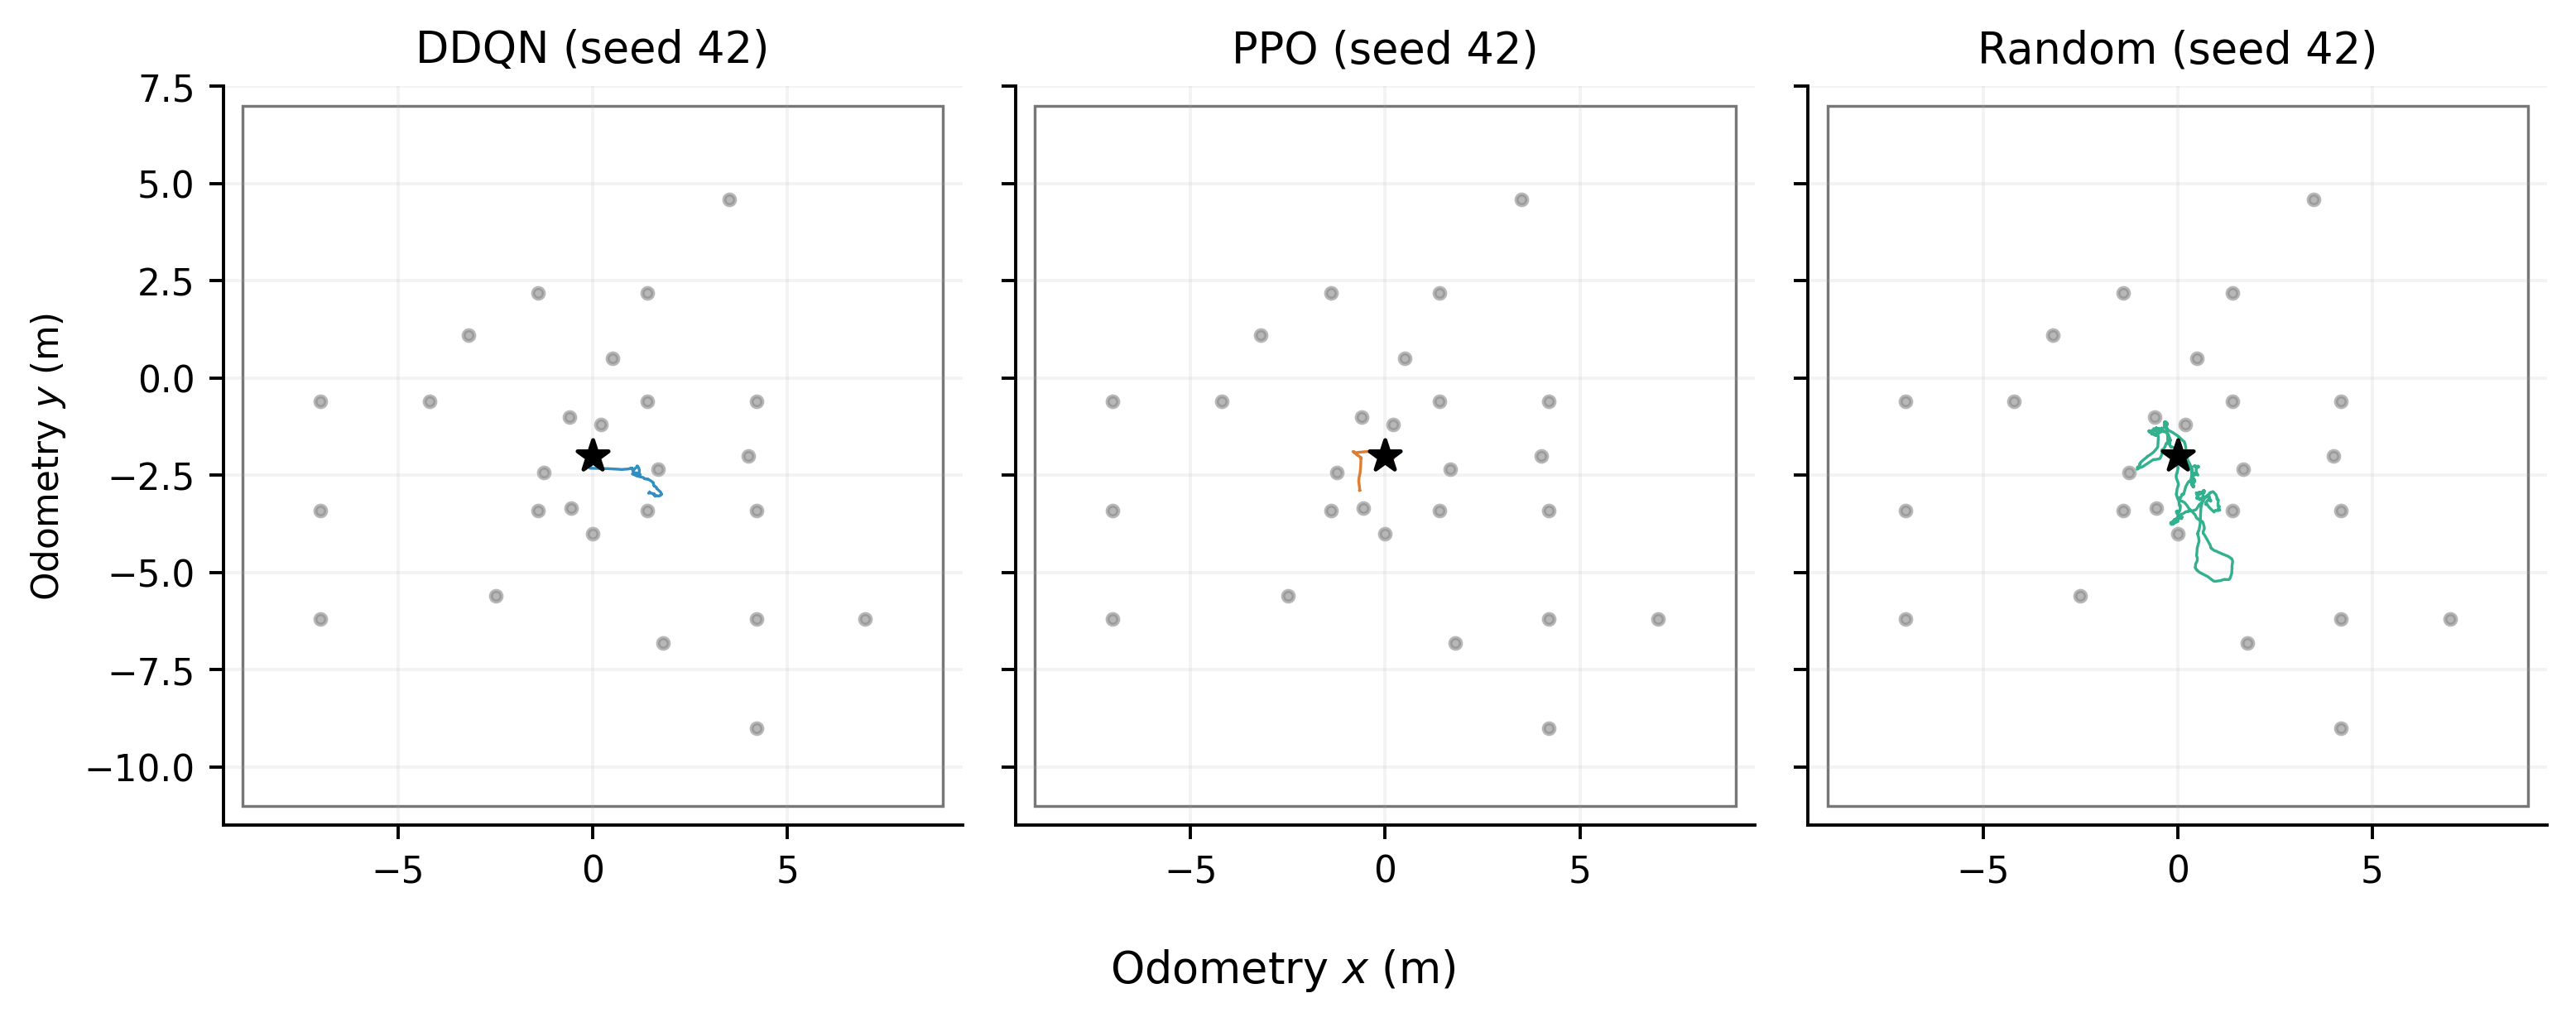
\includegraphics[width=0.86\textwidth]{figures/seed42_trajectories.png}
\caption{Saved odometry trajectories for common seed 42 (trial 1); grey points mark SDF target coordinates for context. DDQN and PPO reached 26/26; Random reached 23/26. The approximate coordinate alignment follows the fixed launch start pose.}
\label{fig:traj}
\end{figure*}

\section{Discussion}
The final records show a substantial \emph{system-level} difference between the assisted configurations and unassisted Random in this world. Assisted systems had high average matching coverage and more complete trials. DDQN had two more full completions than PPO, but their mean counts and successful times were close, and the success intervals overlap. The experiment does not isolate intrinsic DDQN-versus-PPO performance.

The action-source audit changes interpretation more strongly than the aggregate ranking. SLAM coverage, confirmation turns, and sweeps generated almost all applied learned-configuration actions; Random received none of these. The observed gap may arise from those routines, trained policies, detector interaction, or their combination. The planner does not use target ground-truth positions, so its assistance remains an autonomous map-based behavior, but it is a material treatment difference. Uniform random motion is an informative unassisted baseline, not an equal-assistance policy benchmark.

The detection metric also has a narrow meaning. It accepts repeated observations that form a same-class cluster near a known world position. Class-dependent thresholds and a 1.25-m match radius can admit false matches or miss actual instances; two-frame confirmation reduces duplicates but is not manual instance verification. Detector-only accuracy on the final 26-target world was not independently measured. Seed-42 assisted runs matching all targets while moving only locally further illustrates that discovery here measures visual/world matching, not complete physical traversal.

\section{Limitations and Future Work}
This study uses one deliberately spaced 26-object Gazebo world, one start pose, one detector stack, and 17 seed values per method. Results may not transfer to cluttered rooms, new lighting, moving objects, or physical robots. Aligned nominal seeds do not guarantee bitwise-reproducible simulation and perception. Training conditions differ between the final policies, and DDQN stopped short of its requested step count. The short PPO training record and limited DDQN episode summaries do not establish learning dynamics.

The main limitation is unequal assistance. A future factorial study should evaluate each policy with and without the same coverage, inspection, confirmation, and safety modules, with matched training budgets and multiple worlds. Further work should manually audit image-to-world matches, directly estimate false-match and missed-instance rates, and test sensor/map noise. Physical-robot trials would be needed to assess transfer beyond simulation.

\FloatBarrier
\section{Conclusion}
An integrated ROS 2--Gazebo system combined simulated RGB--depth perception, YOLO11n detection, 372-dimensional policy observations, and world-frame instance scoring. Across 51 verified final trials, assisted DDQN and PPO averaged 25.41 and 25.24 of 26 matched objects, versus 19.35 for unassisted Random; their full-discovery counts were 11, 9, and 1. Mean successful completion times were approximately 3.02, 3.05, and 6.94 minutes. Because assistance supplied nearly all realized DDQN/PPO actions, the evidence establishes performance of the complete evaluated configurations in one simulated world rather than a causal ranking of the policies. Equal-assistance ablations and independent match validation are the next essential tests.

\begin{thebibliography}{99}
\bibitem{yamauchi1997} B. Yamauchi, ``A frontier-based approach for autonomous exploration,'' in \emph{Proc. IEEE Int. Symp. Computational Intelligence in Robotics and Automation}, 1997, pp. 146--151.
\bibitem{chaplot2020} D. S. Chaplot, D. Gandhi, S. Gupta, A. Gupta, and R. Salakhutdinov, ``Learning to explore using Active Neural SLAM,'' in \emph{Proc. Int. Conf. Learning Representations}, 2020. [Online]. Available: \url{https://arxiv.org/abs/2004.05155}
\bibitem{mnih2015} V. Mnih \emph{et al.}, ``Human-level control through deep reinforcement learning,'' \emph{Nature}, vol. 518, pp. 529--533, 2015, doi: 10.1038/nature14236.
\bibitem{vanhasselt2016} H. van Hasselt, A. Guez, and D. Silver, ``Deep reinforcement learning with Double Q-learning,'' in \emph{Proc. 30th AAAI Conf. Artificial Intelligence}, 2016, doi: 10.1609/aaai.v30i1.10295.
\bibitem{schulman2017} J. Schulman, F. Wolski, P. Dhariwal, A. Radford, and O. Klimov, ``Proximal policy optimization algorithms,'' arXiv:1707.06347, 2017. [Online]. Available: \url{https://arxiv.org/abs/1707.06347}
\bibitem{raffin2021} A. Raffin, A. Hill, A. Gleave, A. Kanervisto, M. Ernestus, and N. Dormann, ``Stable-Baselines3: Reliable reinforcement learning implementations,'' \emph{J. Mach. Learn. Res.}, vol. 22, no. 268, pp. 1--8, 2021.
\bibitem{redmon2016} J. Redmon, S. Divvala, R. Girshick, and A. Farhadi, ``You only look once: Unified, real-time object detection,'' in \emph{Proc. IEEE Conf. Computer Vision and Pattern Recognition}, 2016, pp. 779--788, doi: 10.1109/CVPR.2016.91.
\bibitem{ultralyticsmodels} Ultralytics, ``YOLO models documentation,'' [Online]. Available: \url{https://docs.ultralytics.com/models/}. Accessed: Nov. 23, 2026.
\bibitem{macenski2022} S. Macenski, T. Foote, B. Gerkey, C. Lalancette, and W. Woodall, ``Robot Operating System 2: Design, architecture, and uses in the wild,'' \emph{Science Robotics}, vol. 7, no. 66, 2022, doi: 10.1126/scirobotics.abm6074.
\bibitem{koenig2004} N. Koenig and A. Howard, ``Design and use paradigms for Gazebo, an open-source multi-robot simulator,'' in \emph{Proc. IEEE/RSJ Int. Conf. Intelligent Robots and Systems}, 2004, pp. 2149--2154, doi: 10.1109/IROS.2004.1389727.
\bibitem{macenski2021slam} S. Macenski and I. Jambrecic, ``SLAM Toolbox: SLAM for the dynamic world,'' \emph{J. Open Source Softw.}, vol. 6, no. 61, p. 2783, 2021, doi: 10.21105/joss.02783.
\bibitem{osrfmodels} Open Robotics, ``Gazebo model database,'' GitHub repository. [Online]. Available: \url{https://github.com/osrf/gazebo_models}. Local checkout: \texttt{8163eb4b5e7e21985c6591d1c0bfb56468c0093f}.
\bibitem{projectrepo} G. R. Thatipamula, ``ROS\_PROJECT: Robot exploration source and final 26-object world,'' GitHub repository. [Online]. Available: \url{https://github.com/Granthik6/ROS_PROJECT/blob/main/src/robot_tasks/worlds/spaced_objects_reliable_26_v4.world}. Accessed: Nov. 23, 2026.
\bibitem{wilson1927} E. B. Wilson, ``Probable inference, the law of succession, and statistical inference,'' \emph{J. Amer. Statist. Assoc.}, vol. 22, no. 158, pp. 209--212, 1927, doi: 10.1080/01621459.1927.10502953.
\end{thebibliography}

\end{document}
